\documentclass[xcolor=table]{beamer}
\usepackage{newclude}
\usepackage{amsfonts,amsmath,oldgerm}
\usepackage[utf8]{inputenc}
\usepackage[T1]{fontenc}
\usepackage{graphicx}
\usepackage[utf8]{inputenc}
\usepackage{amsmath}
\usepackage{amssymb,amsfonts,latexsym,cancel}
\usepackage{listings}
\usepackage{graphicx}
\usepackage{xcolor}
\usepackage[normalem]{ulem}
\usepackage{multicol}
\usepackage{multirow}
\usepackage{booktabs}
\usepackage{listingsutf8}
\usepackage{hyperref}
\usepackage{subfig}
\usepackage{verbatim}
\usepackage{datetime}
\usepackage{pifont}
\usepackage[export]{adjustbox}
\usepackage{hyperref}

\usepackage[
  backend=biber,
  style=ieee,
  url=false,
  doi=true,
  isbn=false
]{biblatex}
\addbibresource{bibliography.bib}

\includeonly{
    Introduction,
    Perspective,
    Homographies,
    Panoramic,
    Dental
}

\usetheme{sintef}

\newcommand{\testcolor}[1]{\colorbox{#1}{\textcolor{#1}{test}}~\texttt{#1}}

\usefonttheme[onlymath]{serif}

\titlebackground*{assets/logo_titlepage}

\newcommand{\hrefcol}[2]{\textcolor{cyan}{\href{#1}{#2}}}

\title{Projective geometry and Panoramic image}
\subtitle{Image Processing, Analysis and Classification}

\author{Sergio Marín Sánchez}

\newdate{date}{2}{4}{2024}
\date{\displaydate{date}}

\setbeamertemplate{footline}{}

\begin{document}

\thispagestyle{empty}

\maketitle

\section{Introduction}

\begin{frame}{\secname}{3D world $\rightarrow$ 2D content}
    An image is just a flat representation of the 3D world.
    \begin{figure}
        \centering
        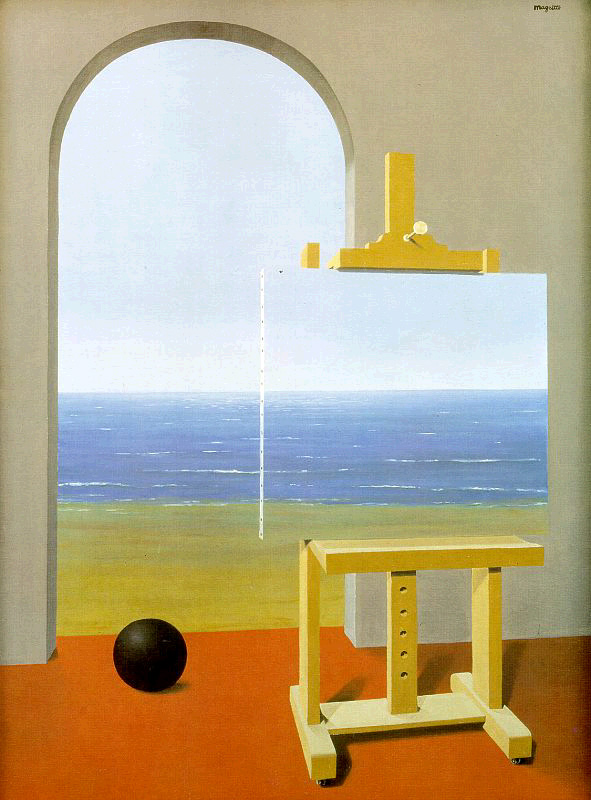
\includegraphics[height=0.5\textheight]{img/Magritte-human-condition.jpg}
    \end{figure}
    Even though we lose the depth component the image maintain the perspective.
\end{frame}

\begin{frame}{\secname}{3D world $\rightarrow$ 2D content}
    Image are useful to store memories, but also we can extract information from them. For instance, we may want to know how tall is this bottle.
    \begin{figure}
        \centering
        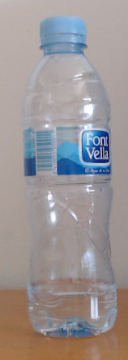
\includegraphics[height=0.5\textheight]{img/agua.png}
    \end{figure}
\end{frame}

\begin{frame}{\secname}{3D world $\rightarrow$ 2D content}
    We need to represent the images in such a way that both humans and computers are able to deal with them. Thus matrix representation of images is defined. We can define an image $I \in M_{h,w}\left(\mathbb{Z}^n\right)$ as:
    \begin{gather*}
        I = \begin{pmatrix}
            p_{1,1} & p_{1,2} & \dots & p_{1,w} \\
            p_{2,1} & p_{2,2} & \dots & p_{2,w} \\
            \vdots & \vdots & \ddots & \vdots \\
            p_{h,1} & p_{h,2} & \dots & p_{h,w} \\
        \end{pmatrix}_{h \times w}
    \end{gather*}
    
    Where each $p_{ij}$ is a vector in $\mathbb{Z}^n$, $n$ varies depending on the number of color channels.
\end{frame}

\begin{frame}{\secname}{3D world $\rightarrow$ 2D content}  
    Here we can see how the image is codified as we have defined before:
    \begin{figure}
        \centering
        \subfloat{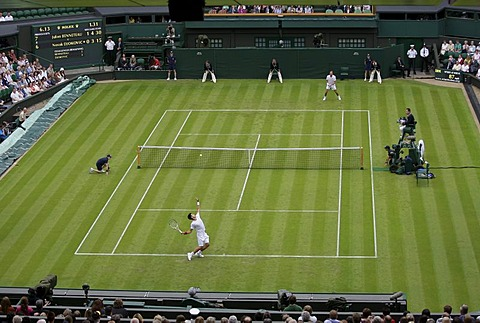
\includegraphics[width=0.4\textwidth]{img/tennis.jpg}}
        \qquad
        \subfloat{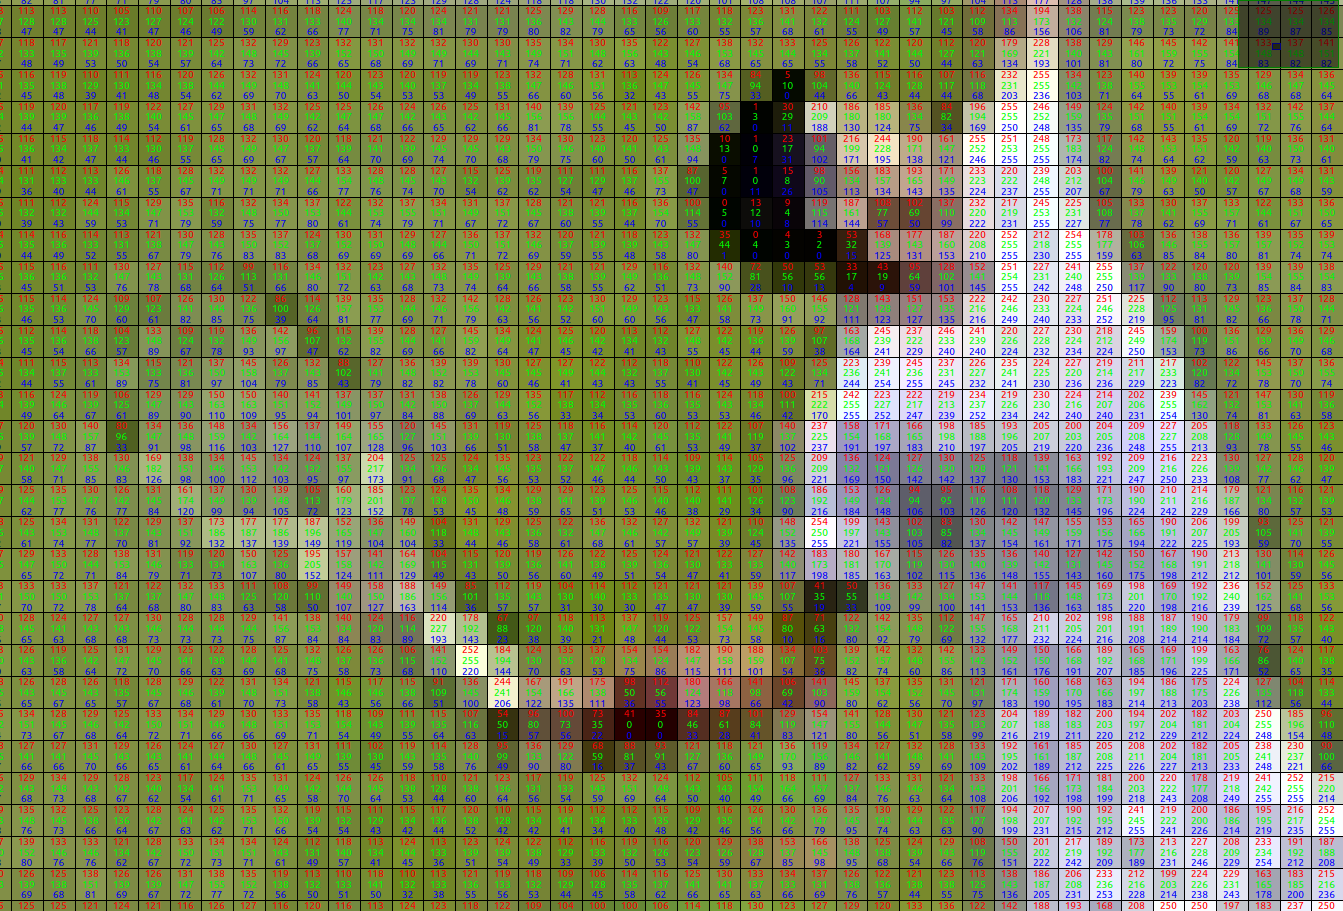
\includegraphics[width=0.4\textwidth]{img/pixels2.png}}
    \end{figure}
\end{frame}



\section{Perspective}

Perspective in digital images is a critical aspect that influences the perception of depth and spatial relationships within a scene. It is primarily manipulated through various parameters, with focal distance being one of the key elements.

The focal distance, often denoted as $f$, is a fundamental parameter in digital imaging that determines the magnification and perspective of the captured scene. It refers to the distance between the lens and the image sensor when the subject is in focus. A shorter focal distance results in a wider field of view, allowing more of the scene to be captured within the frame, while a longer focal distance narrows the field of view, resulting in magnification and compression of distant objects.

By using this focal distance, we can establish different measurements (angles) inside of the image. A potential use case for these measurements is triangulate locations. Firstly, some reference points are selected. Then, calculate the angle between them, two by two. Finally, these angles are placed over a map, and the intersection between them would indicate the actual position where the photo was taken. This method only requires some basic trigonometrics, as it can be seen in Fig. \ref{fig:triangulation}.

\begin{figure}[H]
    \centering
    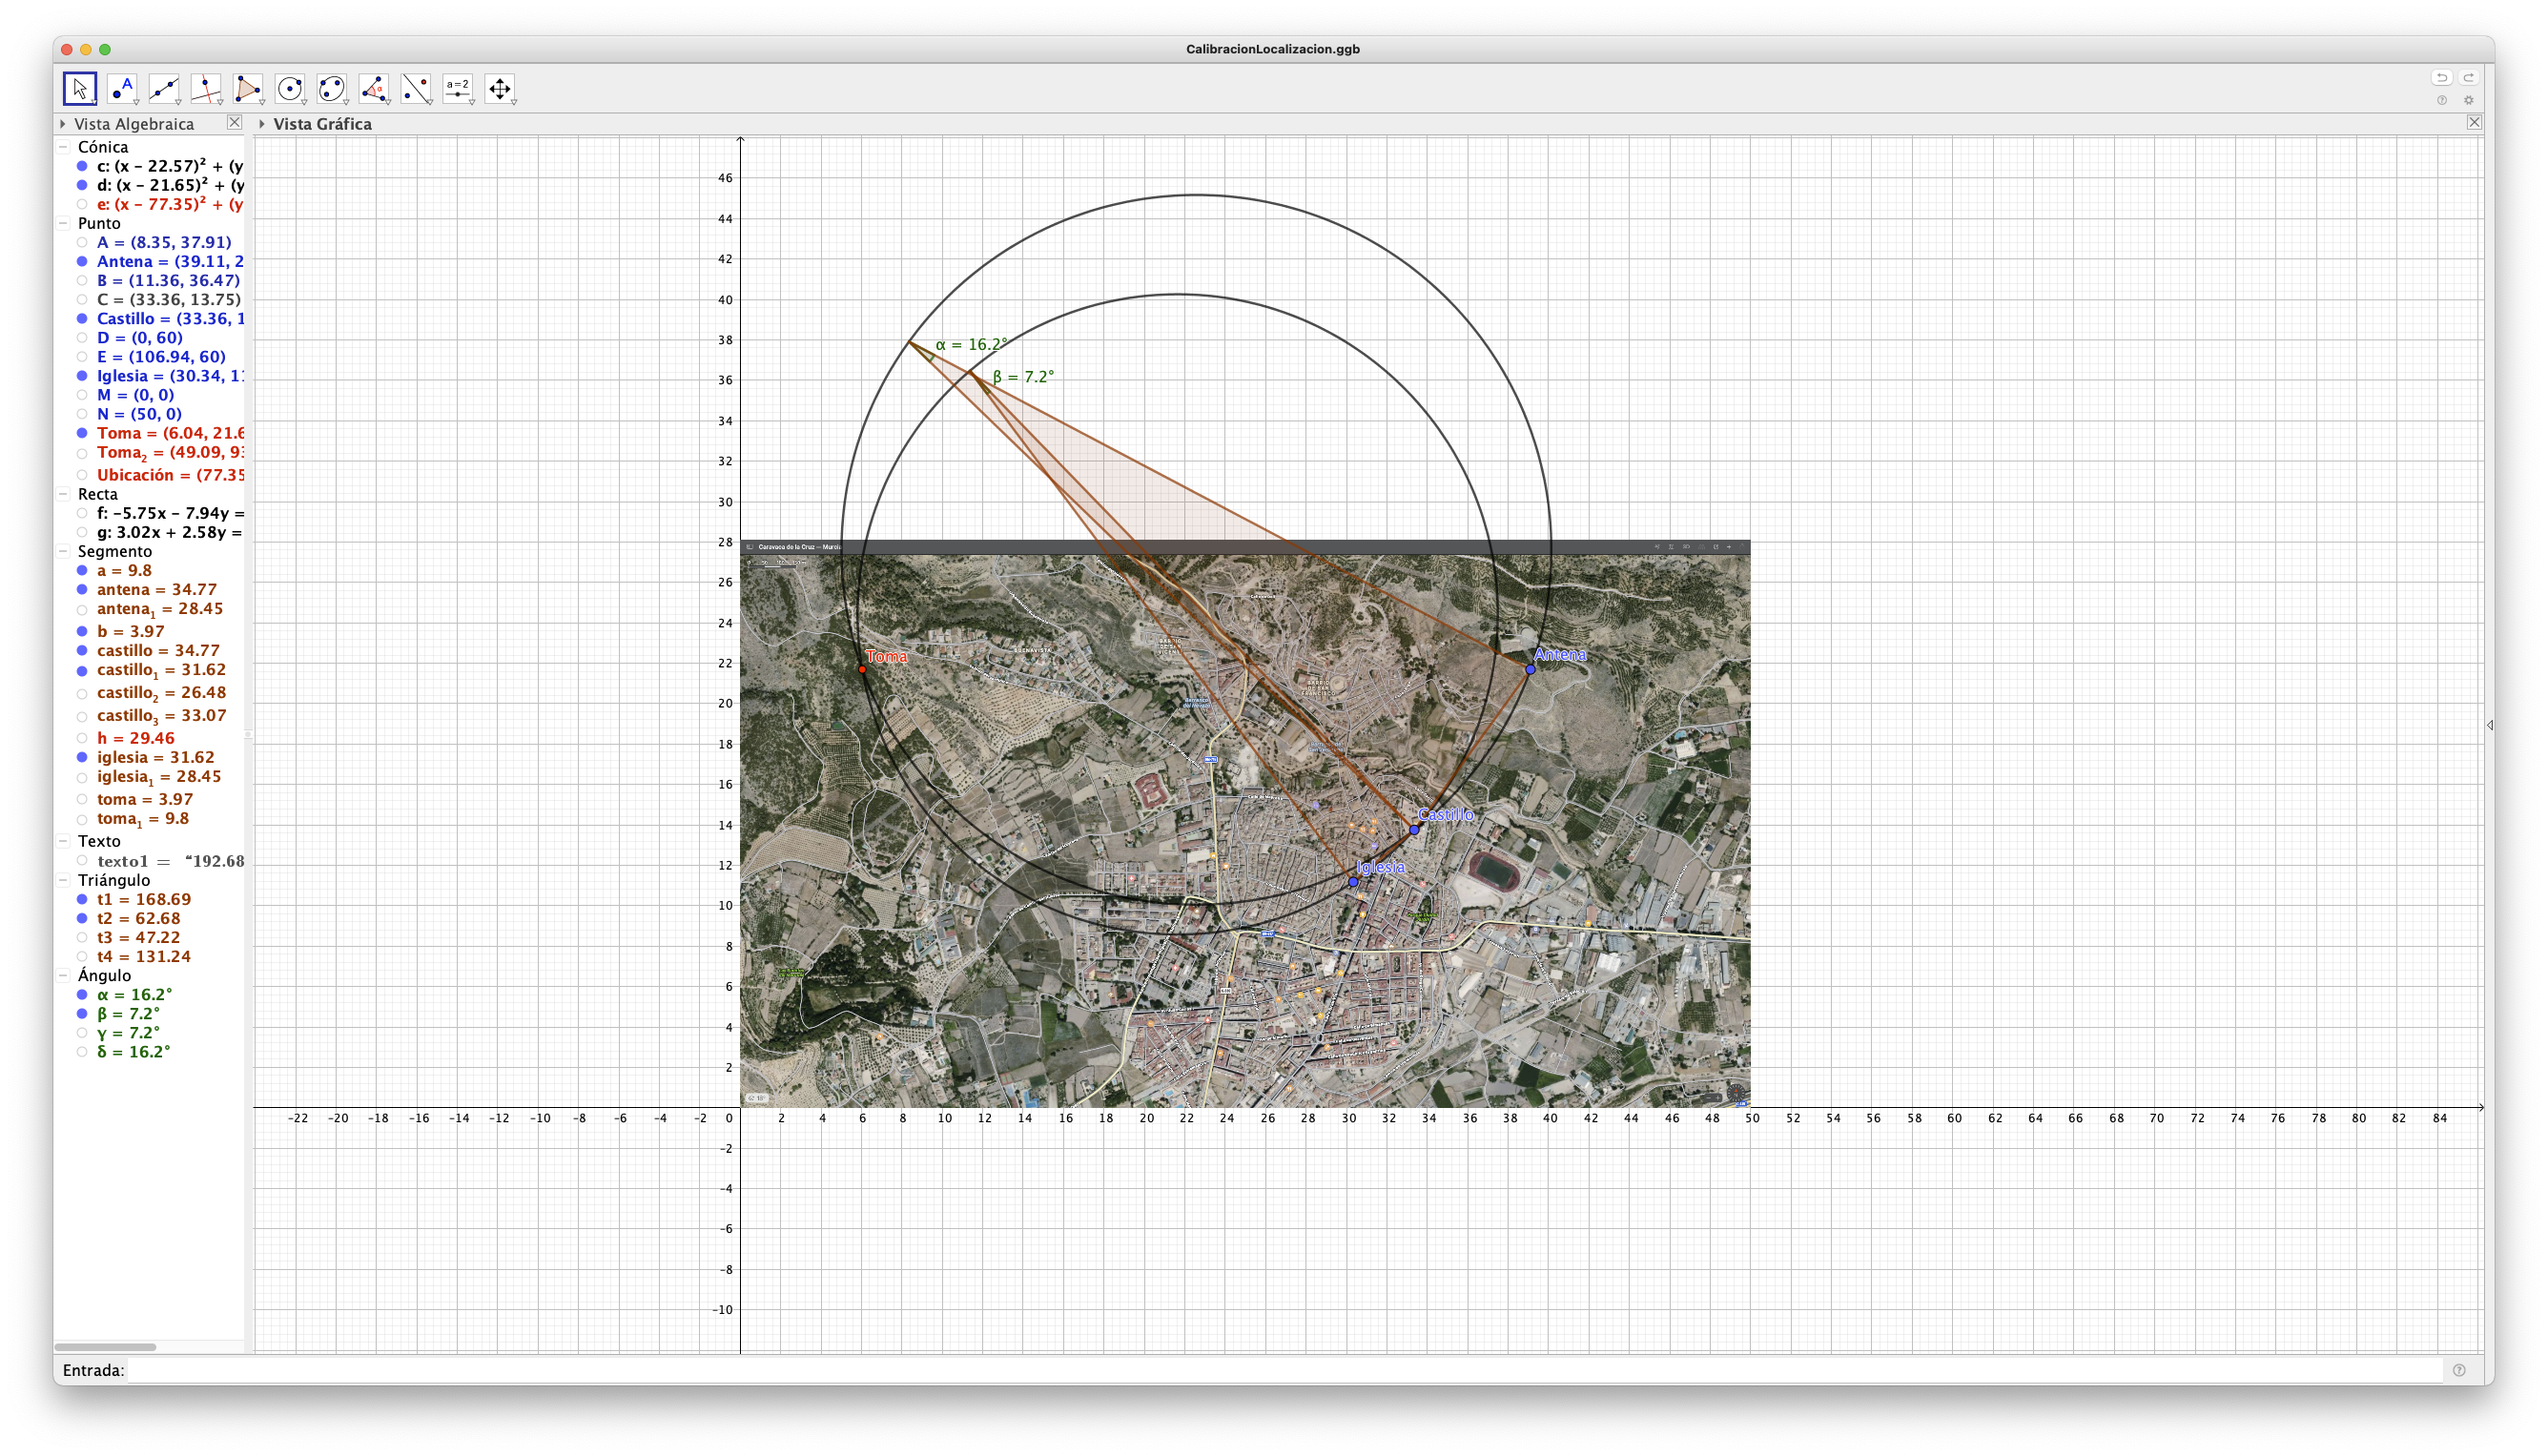
\includegraphics[width=0.9\textwidth]{img/Inter-Circs.png}
    \caption{Example of location triangulation}
    \label{fig:triangulation}
\end{figure}



\section{Homographies}

\begin{frame}{\secname}
    ``The homograph is a mapping between two perspective images of a planar surface in a scene'' \cite{gledhill_panoramic_2003}
    \begin{figure}
        \centering
        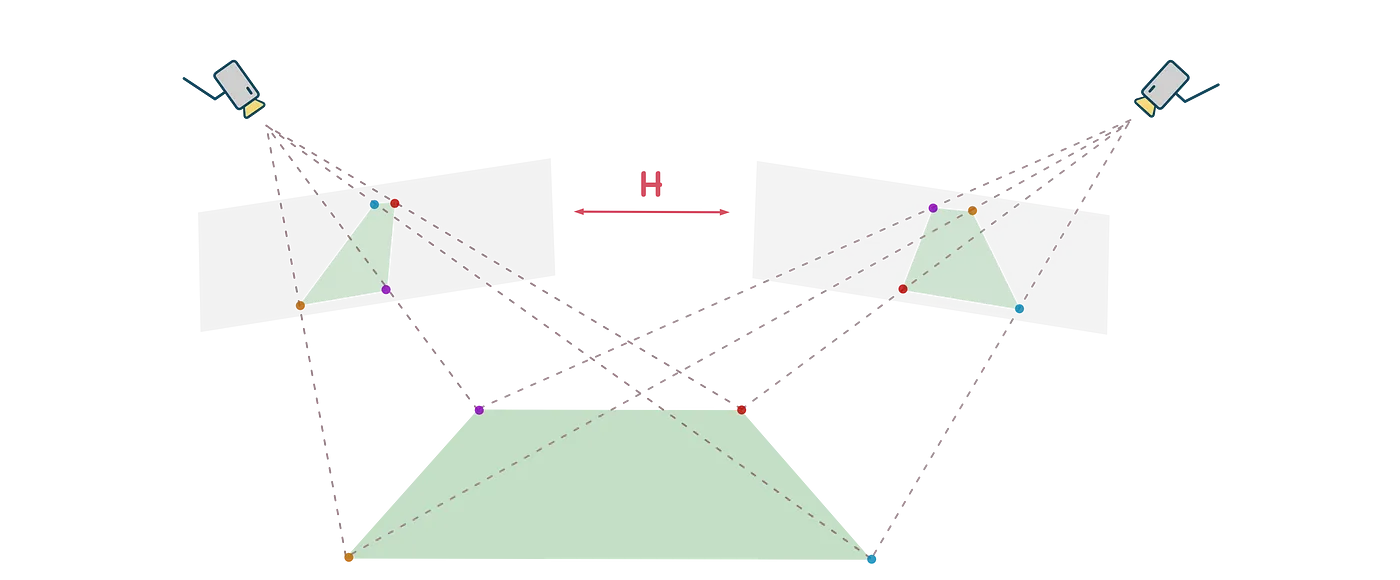
\includegraphics[width=\textwidth]{img/homog}
    \end{figure}
\end{frame}

\begin{frame}{\secname}
    An homography is just a matrix that convert some points into others.
    \begin{gather*}
        \lambda
        \begin{bmatrix}
            x' \\ y' \\ 1
        \end{bmatrix} = 
        \begin{bmatrix}
            H_{1,1} & H_{1,2} & H_{1,3} \\
            H_{2,1} & H_{2,2} & H_{2,3} \\
            H_{3,1} & H_{3,2} & H_{3,3}
        \end{bmatrix}
        \begin{bmatrix}
            x \\ y \\ 1
        \end{bmatrix}
    \end{gather*}    
\end{frame}


\begin{frame}{\secname}{Use case: How far was this shot?}
    By using homographies we can remove the perspective from an image, and after that we can measure in the image.
    \begin{figure}
        \subfloat{\includegraphics[width=0.5\textwidth]{img/puntoshomog_orig}}
        \subfloat{\includegraphics[width=0.4\textwidth]{img/puntoshomog_ref}}
    \end{figure}
\end{frame}

\begin{frame}{\secname}{Use case: How far was this shot?}
    By using homographies we can remove the perspective from an image. 
    \begin{figure}
        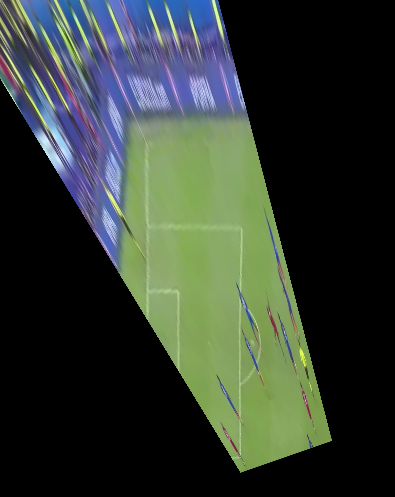
\includegraphics[width=0.5\textheight]{img/homog_eden}
    \end{figure}
\end{frame}

\begin{frame}{\secname}{Use case: How far was this shot?}
    We can establish measurements in the image.
    \begin{figure}
        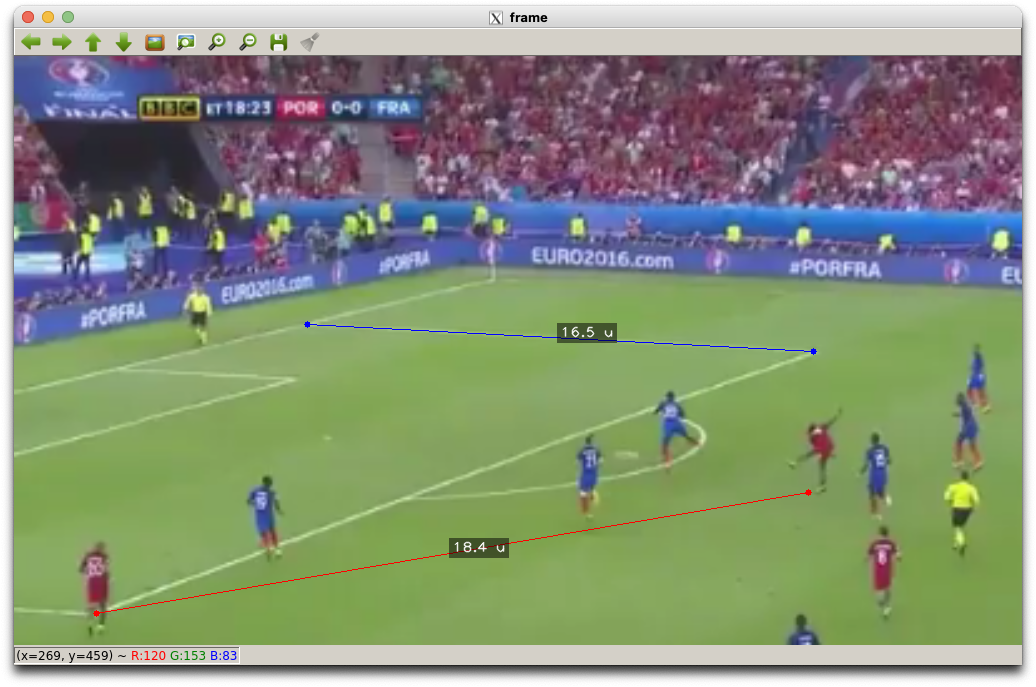
\includegraphics[width=0.7\textheight]{img/Medida_HomogOrig_Final}
    \end{figure}
\end{frame}

\begin{frame}{\secname}{Use case: How far was this shot?}
    Using trigonometry, as before, we can estimate the shot distance.
    \begin{figure}
        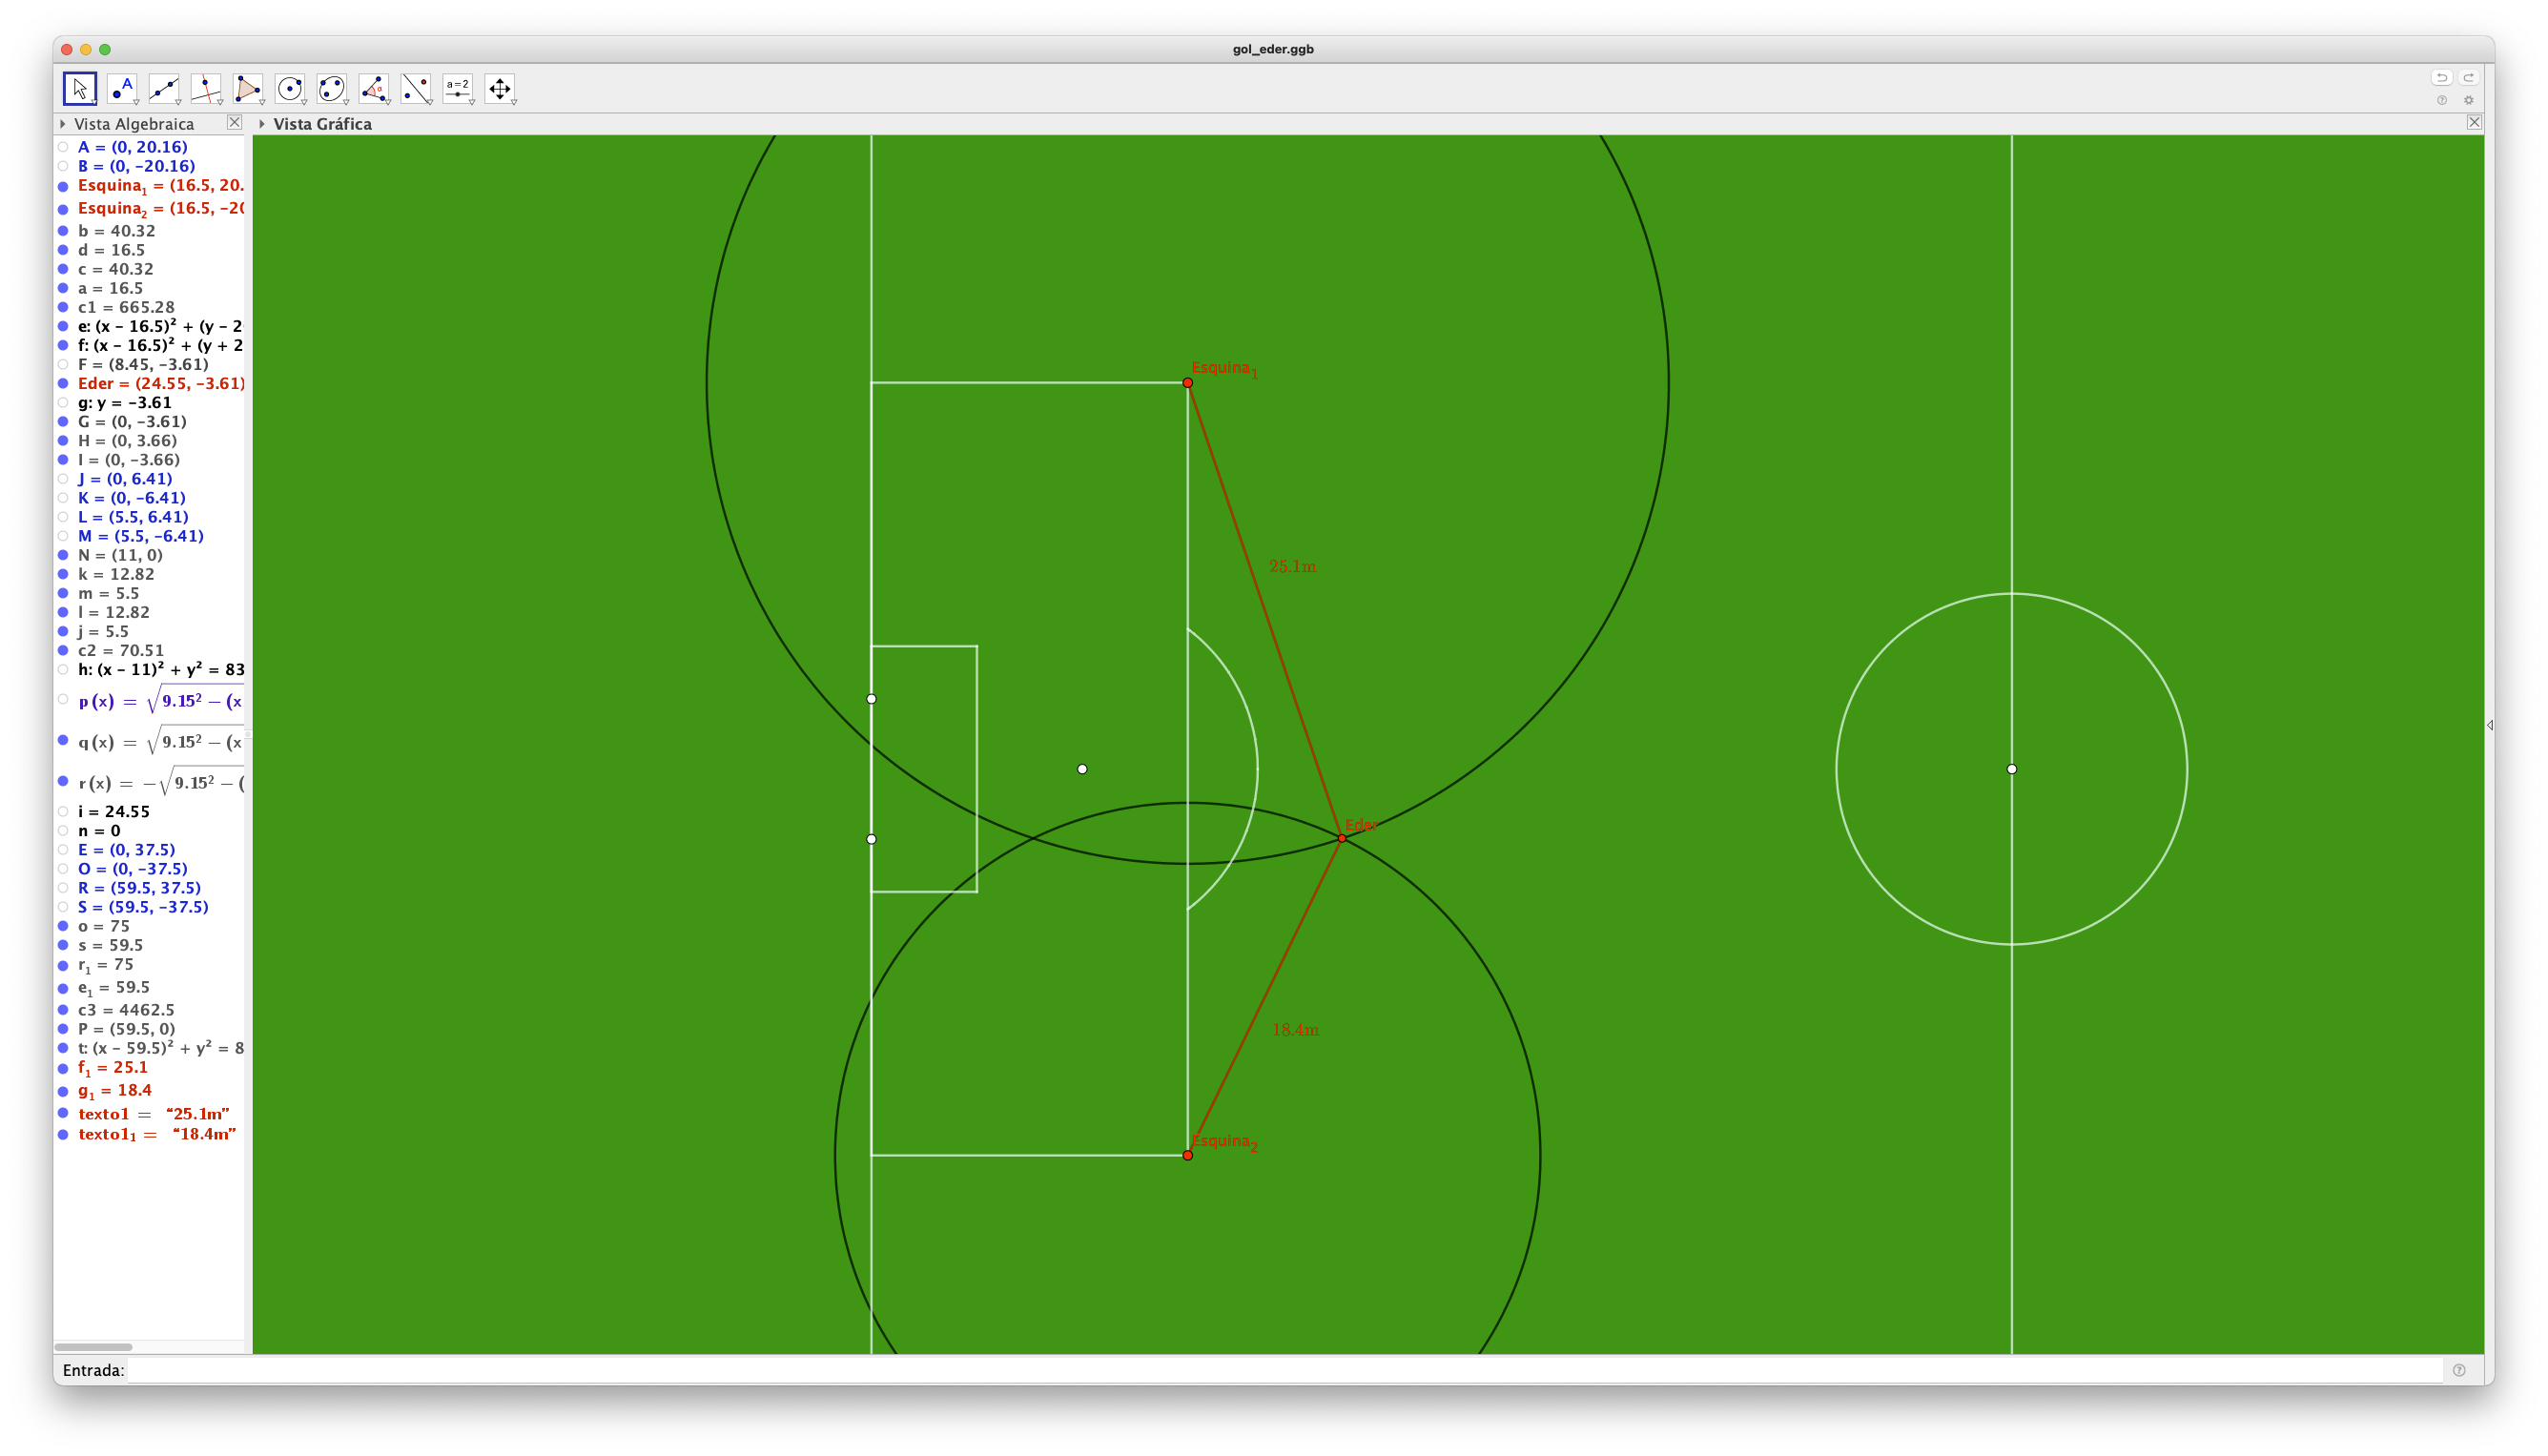
\includegraphics[width=\textwidth]{img/posicion-eder}
    \end{figure}
\end{frame}

\begin{frame}{\secname}{Use case: How far was this shot?}
    Using trigonometry, as before, we can estimate the shot distance.
    \begin{figure}
        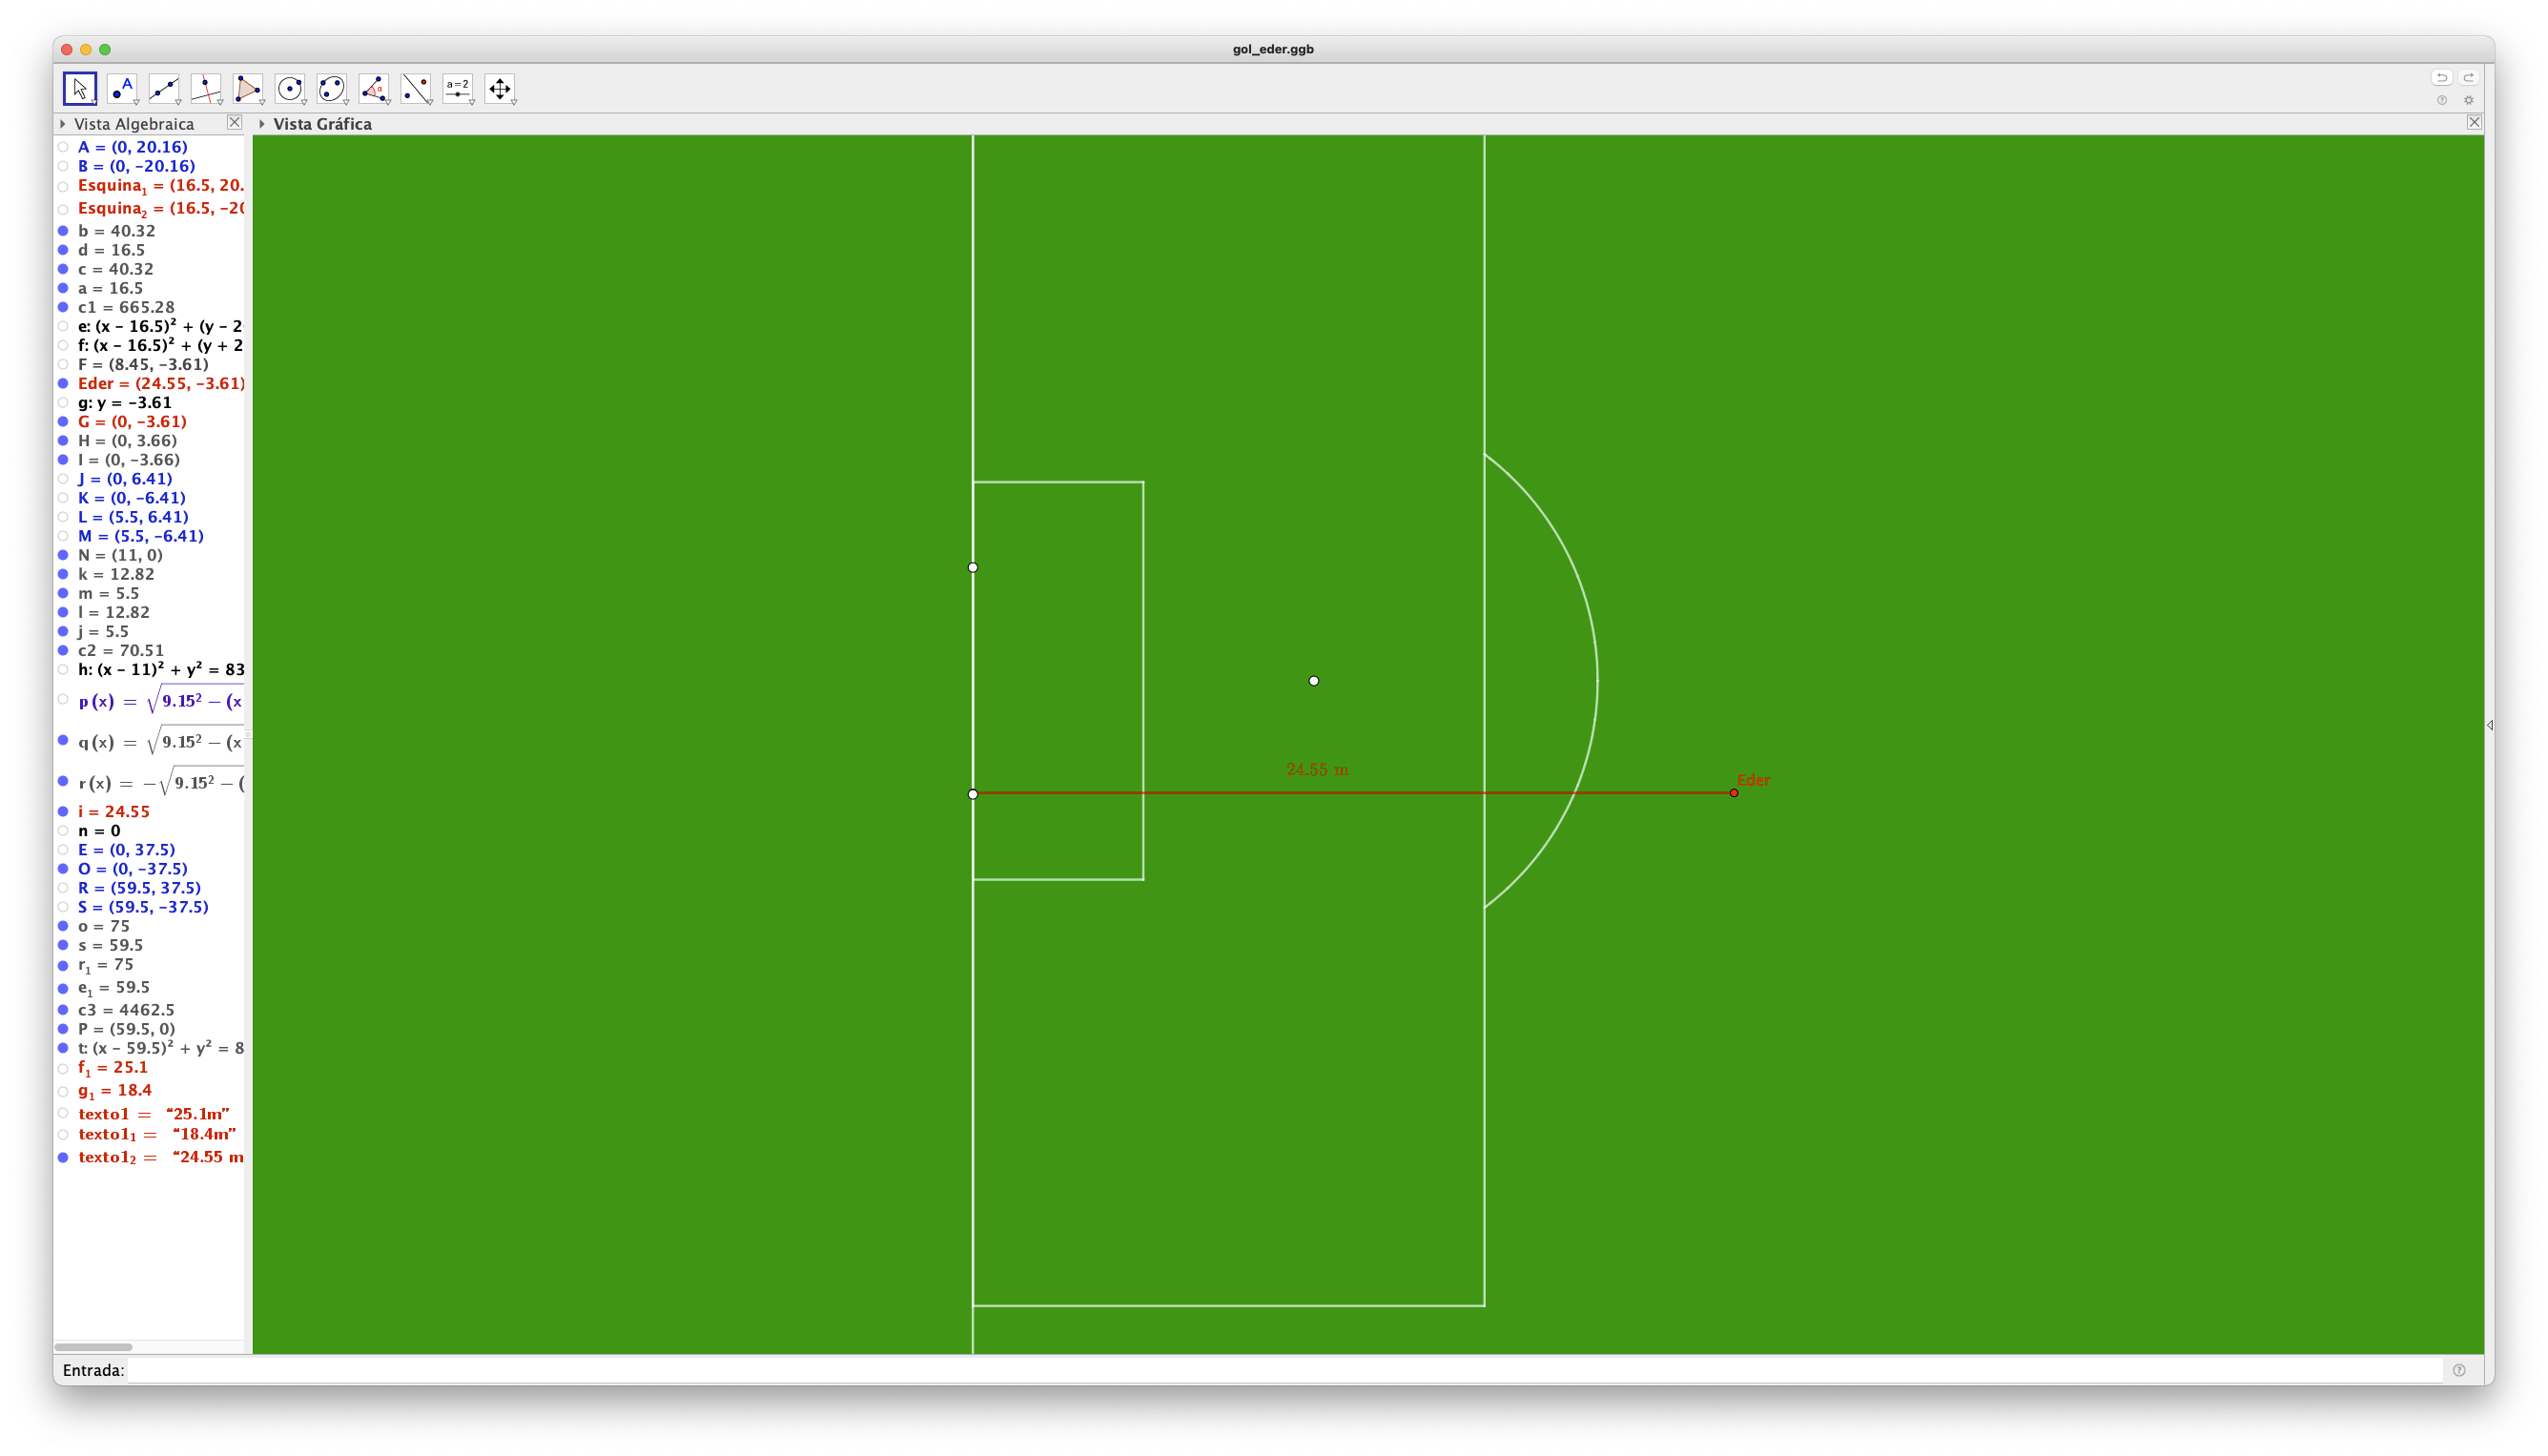
\includegraphics[width=\textwidth]{img/medida-eder}
    \end{figure}
\end{frame}



\section{Panoramic image}

\begin{frame}{\secname}
    Panoramic image reconstruction uses the techniques explain before.
    \begin{figure}
        \centering
        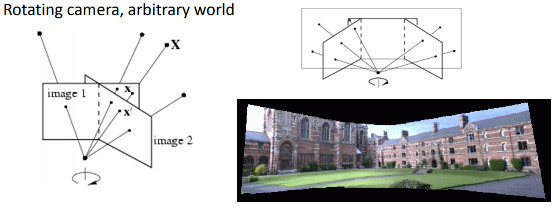
\includegraphics[width=0.8\textwidth]{img/homography_transformation_example3}
        \caption{Panoramic image reconstruction \cite{noauthor_opencv_nodate}}
    \end{figure}
\end{frame}

\begin{frame}{\secname}
    The key points have to be automatically calculated.
    \begin{figure}
        \centering
        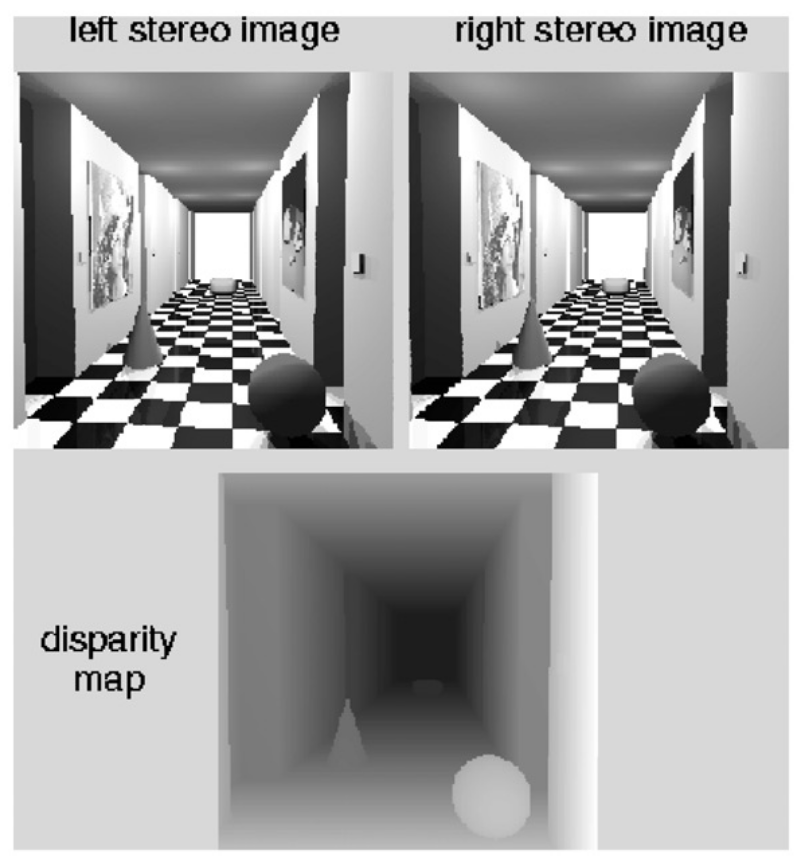
\includegraphics[width=0.5\textheight]{img/pano_make}
        \caption{Stereo images and related disparity map \cite{gledhill_panoramic_2003}}
    \end{figure}
\end{frame}

\begin{frame}{\secname}
    We can use techniques explain during the lessons (Key point feature extraction), such as SIFT, FAST, etc.
    \begin{figure}
        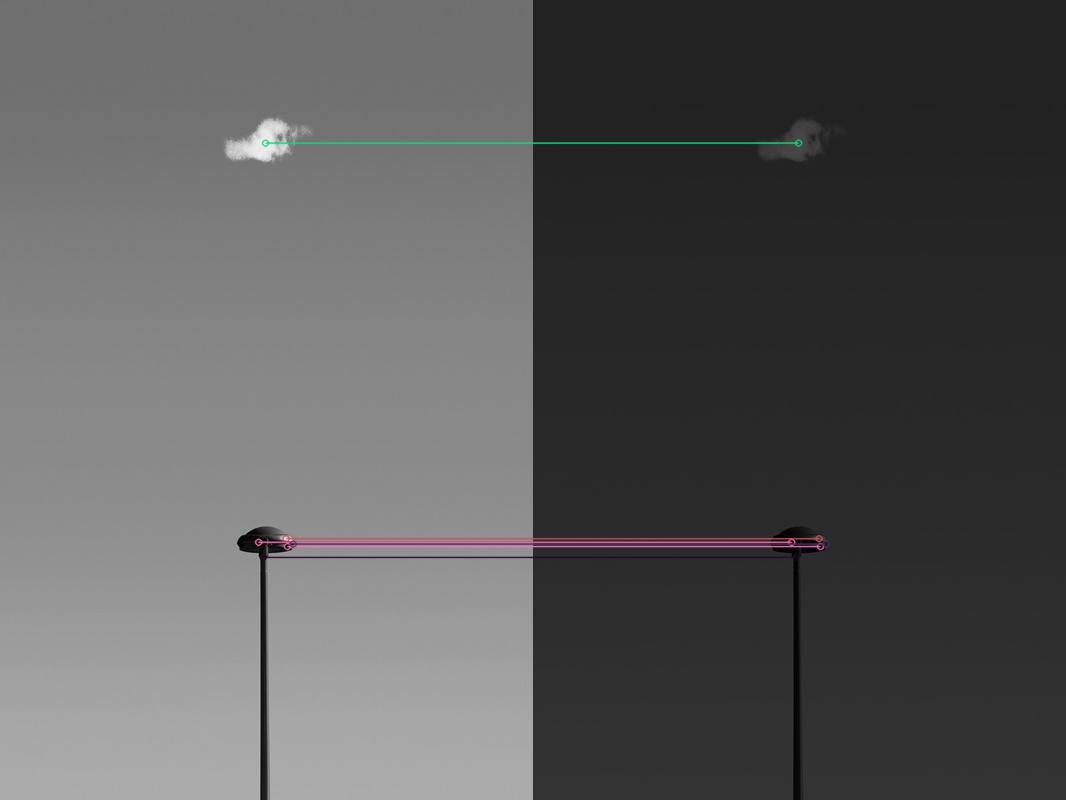
\includegraphics[width=0.5\textwidth]{../doc/sift_algorithm/img/final.png}
        \caption{Key points from practical exercise}
    \end{figure}
\end{frame}

\begin{frame}{\secname}
    If the key points are good enough selected, the results could be quite accurate.
    \begin{figure}
        \centering
        \subfloat[Original images before the mosaic \cite{gledhill_panoramic_2003}]{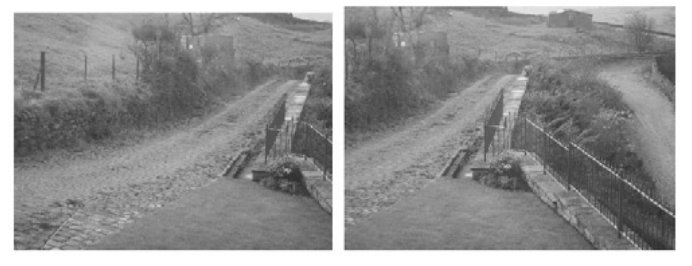
\includegraphics[width=0.5\textwidth]{img/pano_both.png}} \\
        \subfloat[Two images stitched together \cite{gledhill_panoramic_2003}]{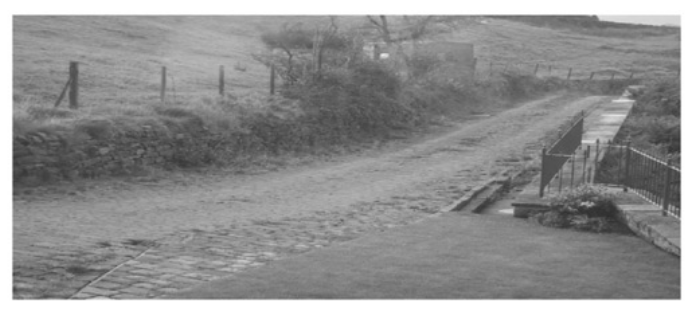
\includegraphics[width=0.5\textwidth]{img/pano_join.png}}
    \end{figure}
\end{frame}

\begin{frame}{\secname}
    This technique can also be used in the reconstruction of non-planar images. \cite{yong_panoramic_2019}
    \begin{figure}
        \centering
        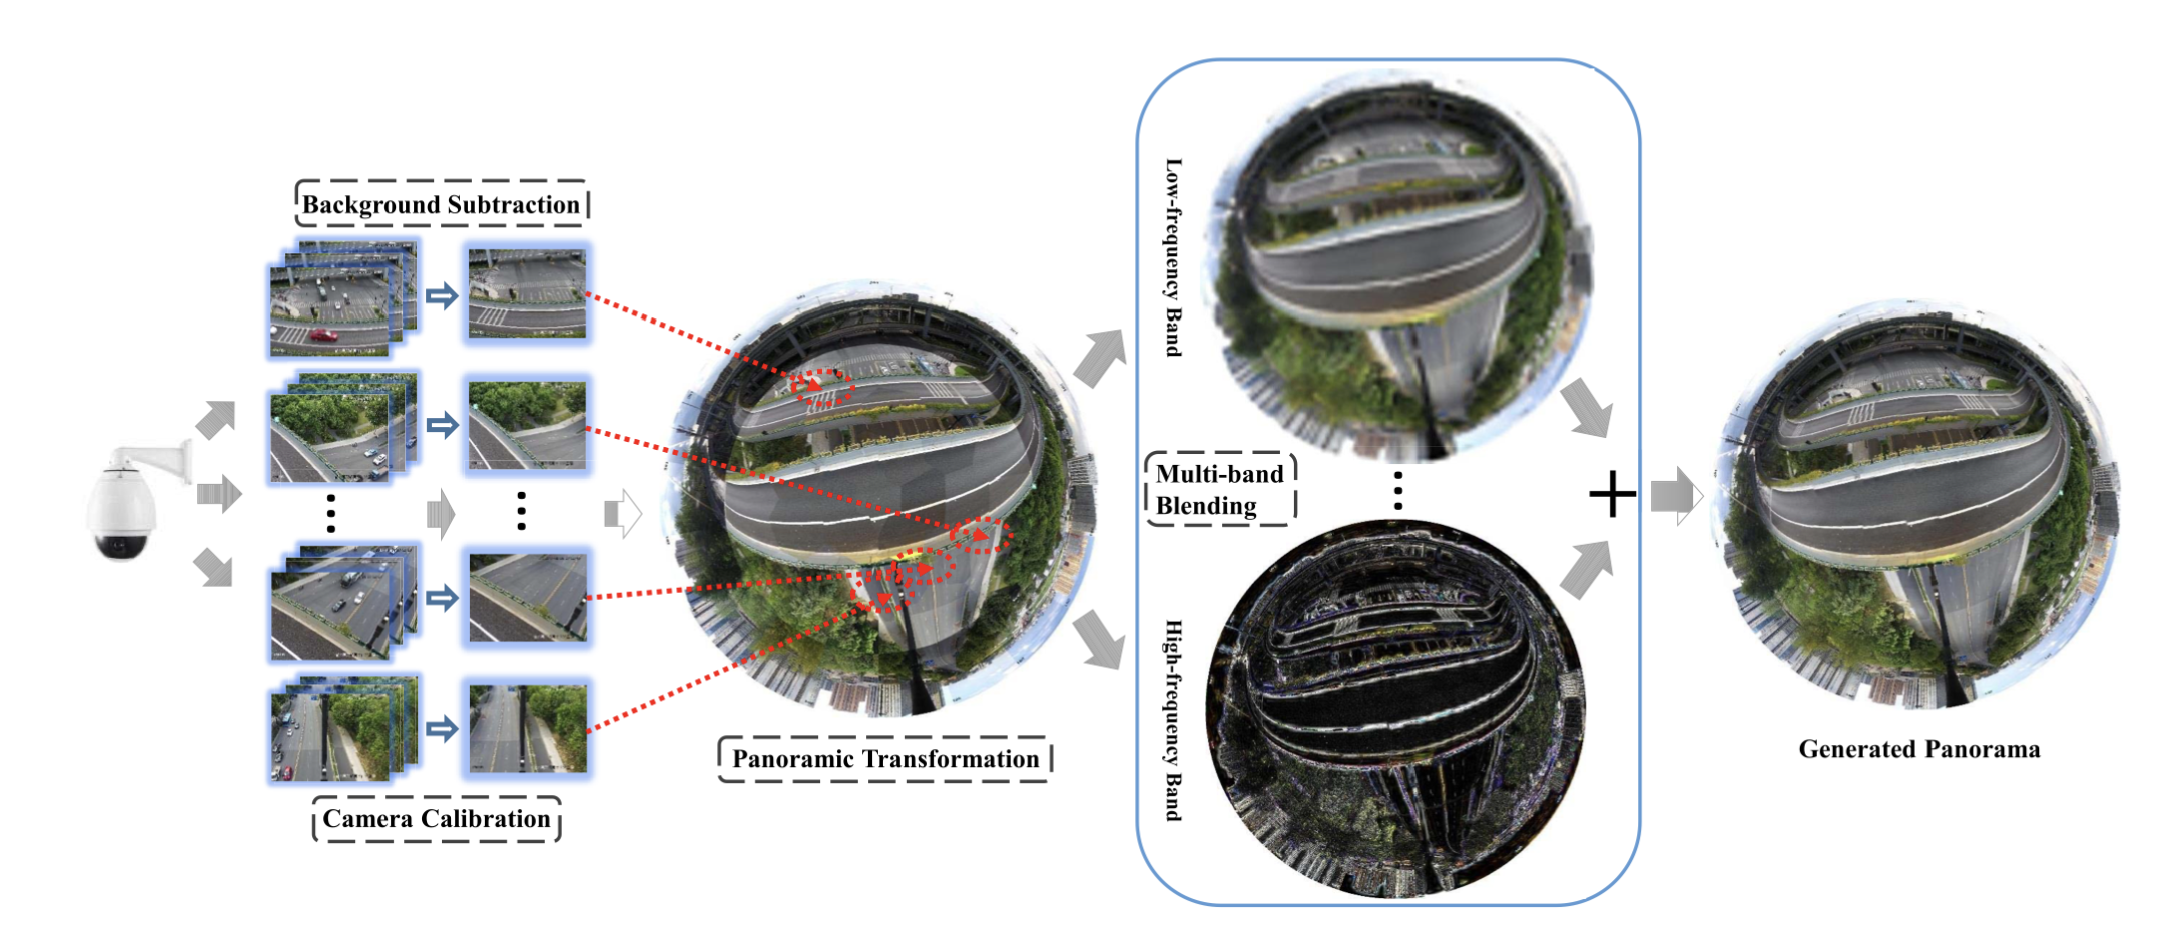
\includegraphics[width=\textwidth]{img/pano_esphere}
    \end{figure}
\end{frame}

\begin{frame}{\secname}
    Another example with a 360º image. \cite{duan_panoramic_2020}
    \begin{figure}
        \centering
        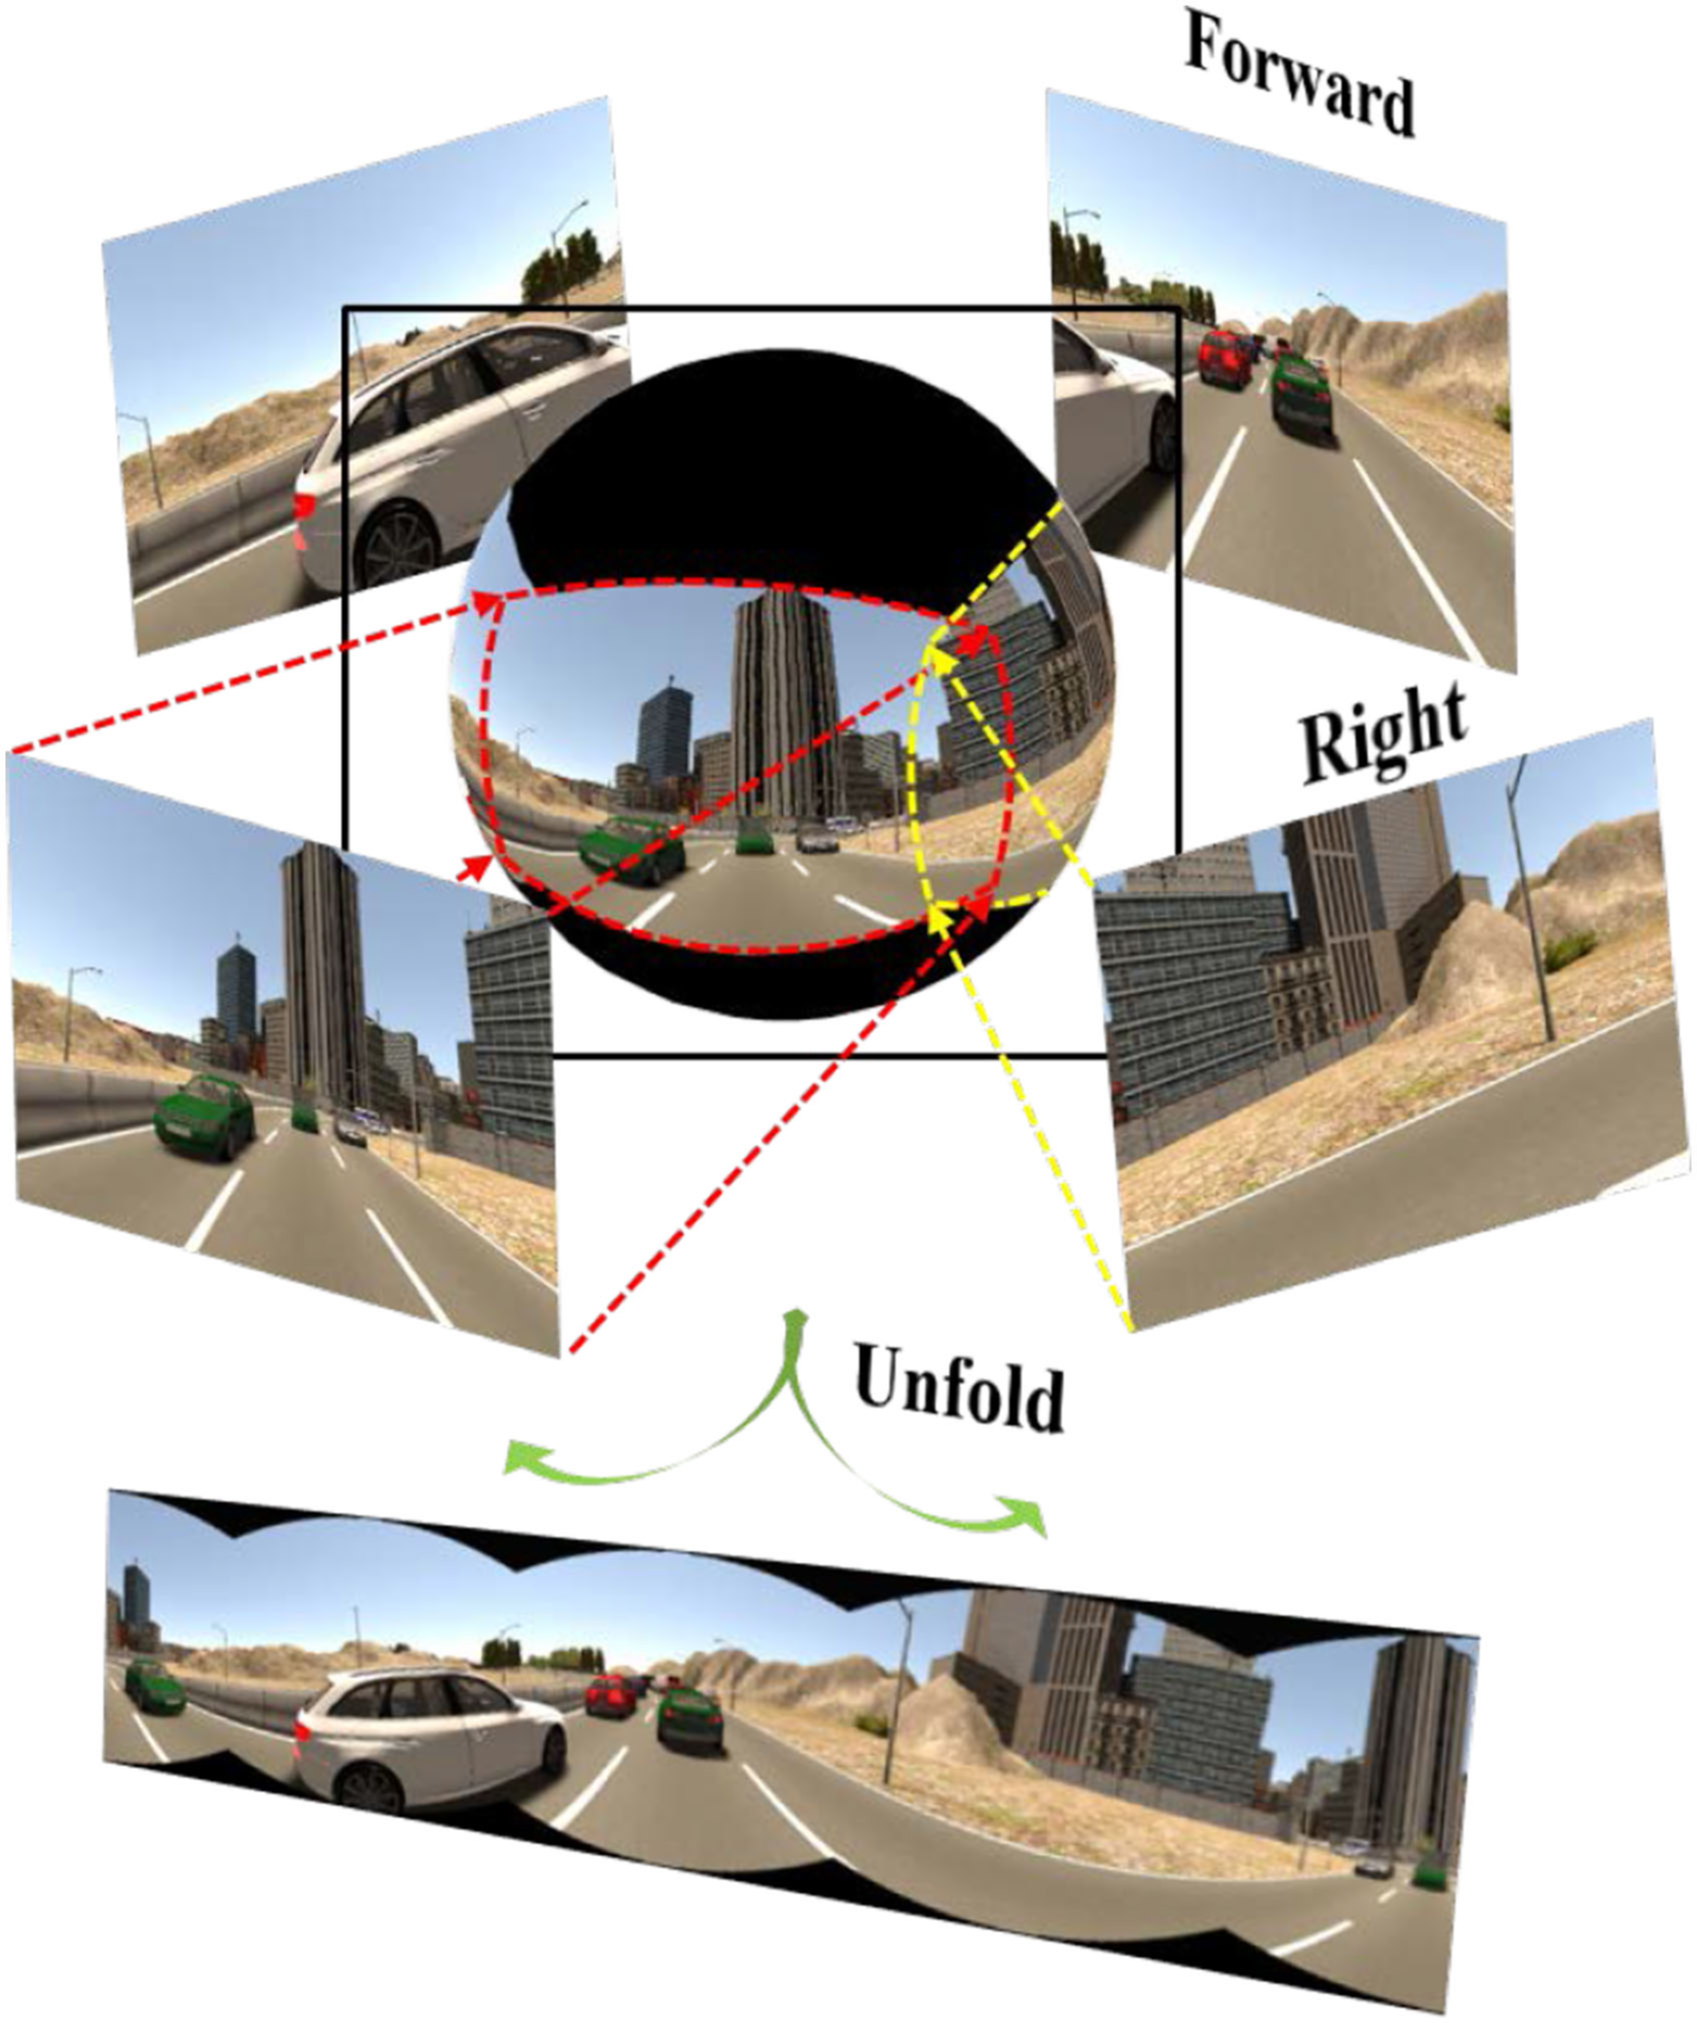
\includegraphics[height=0.7\textheight]{img/duan_esphere}
    \end{figure}
\end{frame}



\section{Use case: Dental images}

\begin{frame}{\secname}{Problem description}
    In the context of dental health, as teeth are bones, the dentist needs to take X-rays.
    \begin{figure}
        \centering
        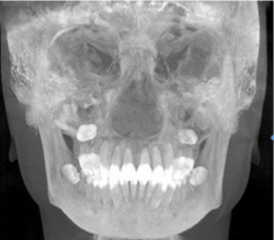
\includegraphics{img/dental_problem}
        \caption{Some teeth hide others \cite{yun_automatic_2019}}
    \end{figure}
\end{frame}

\begin{frame}{\secname}{Proposed solution}
    Yun \textit{et al}. \cite{yun_automatic_2019} came up with a solution based on the contents of this subject.
    \begin{figure}
        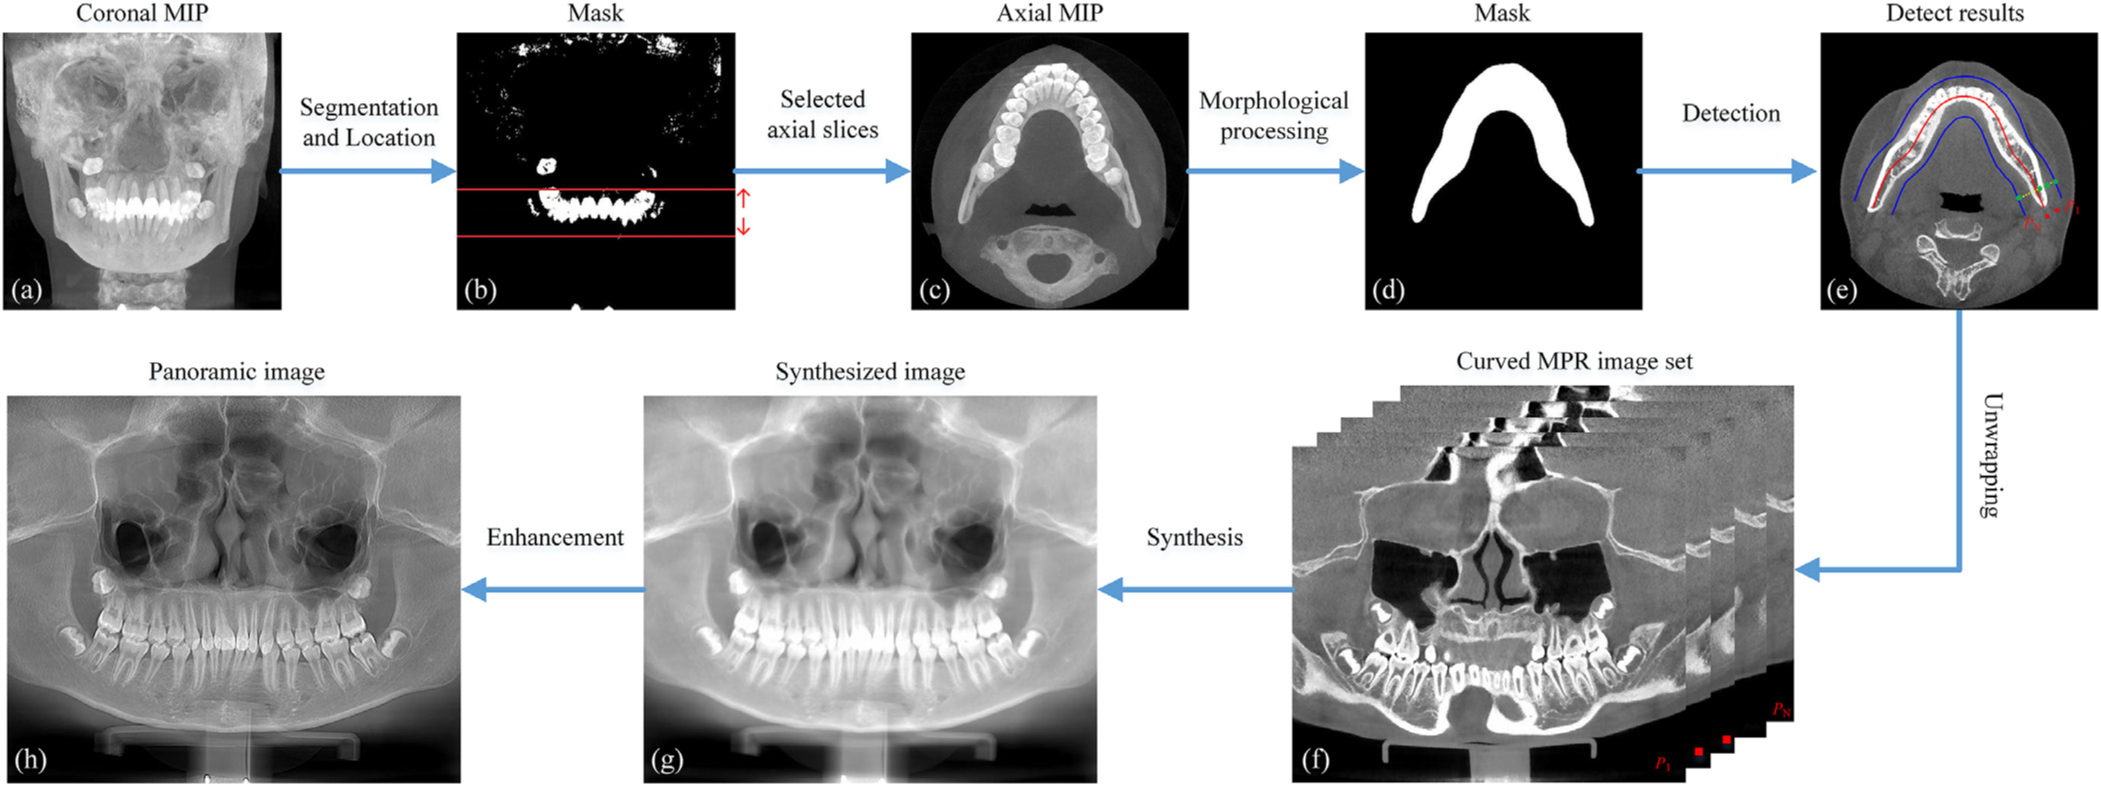
\includegraphics[width=\textwidth]{img/dental_proposal}
    \end{figure} 
\end{frame}

\begin{frame}{\secname}{Thresholding}
    They use histograms to establish a threshold value.
    \begin{figure}
        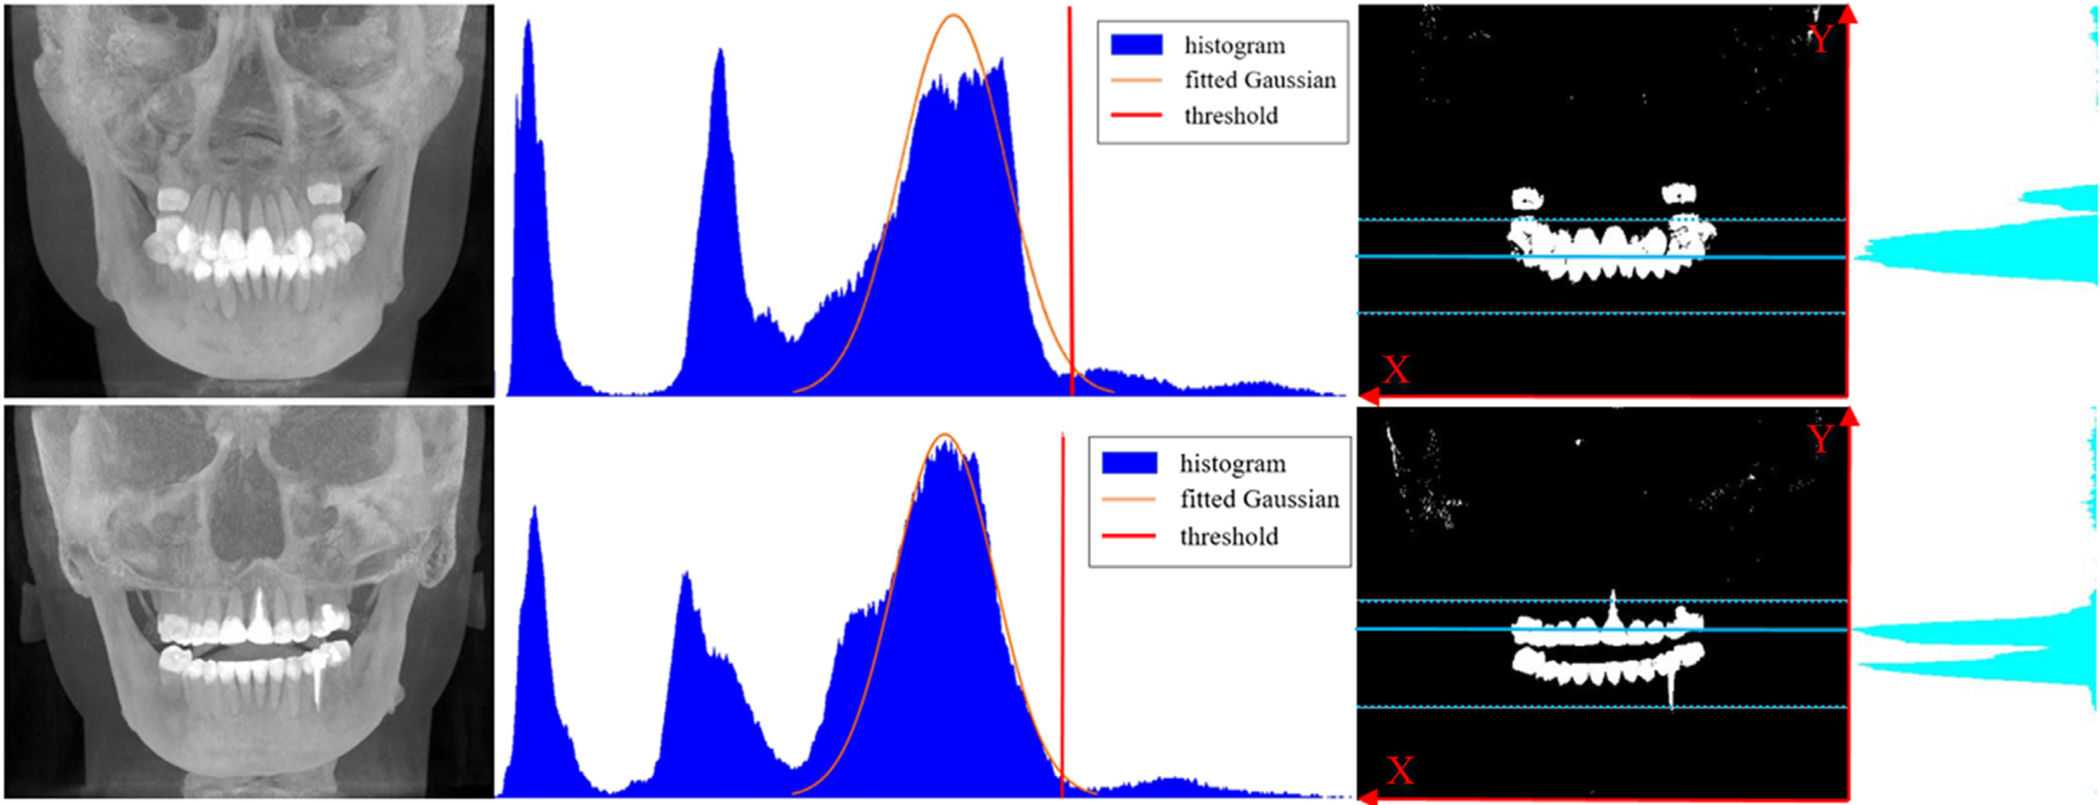
\includegraphics[width=\textwidth]{img/dental_thresh}
    \end{figure} 
\end{frame}

\begin{frame}{\secname}{Morphological processing}
    With the threshold calculated before, they managed to create a mask.
    \begin{figure}
        \centering
        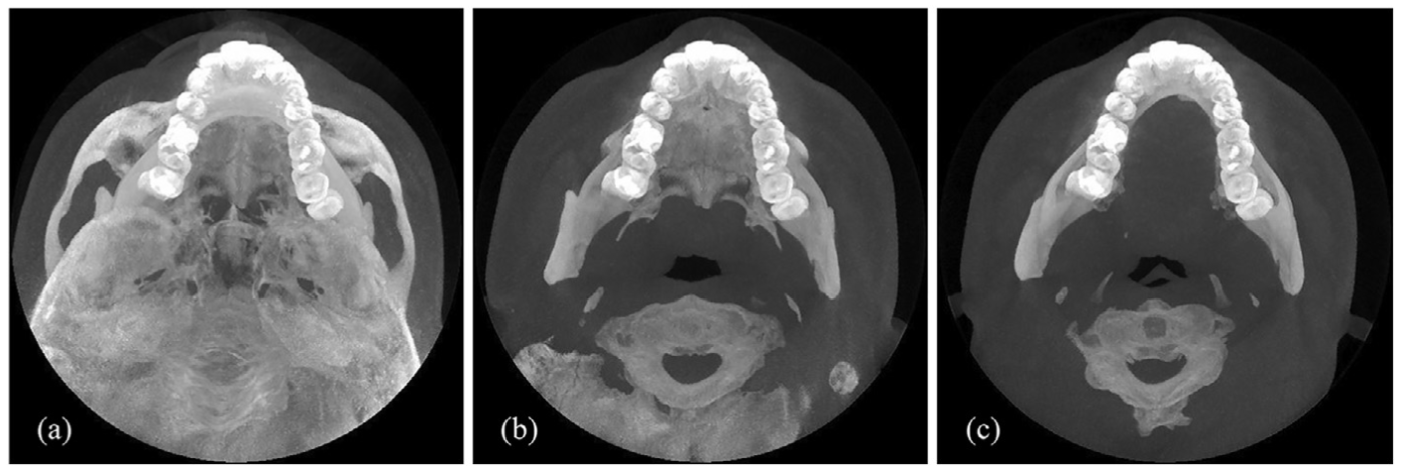
\includegraphics[width=0.7\textwidth]{img/dental_slices}
    \end{figure}
\end{frame}

\begin{frame}{\secname}{Morphological processing}
    With the threshold calculated before, they managed to create a mask.
    \begin{figure}
        \centering
        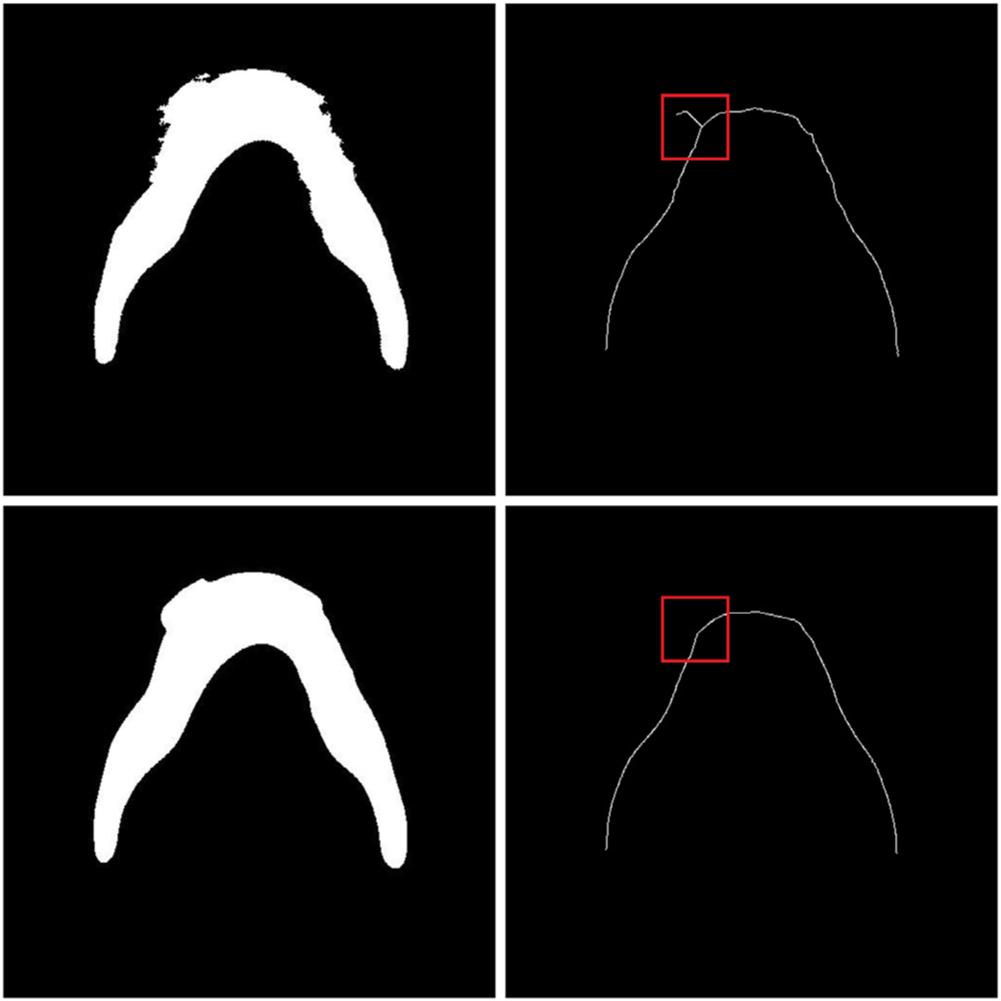
\includegraphics[width=0.3\textwidth]{img/dental_slice_thresh}
    \end{figure}
    Also perform Gaussian filtering
\end{frame}

\begin{frame}{\secname}{Arch approximation}
    Dental arch approximation using the following formula:
    \begin{gather*}
        I_0(i, j) = S \cdot \log \left( \sum_{n=1}^N e^{\frac{P_n(i,j)}{S}} \right)
    \end{gather*}
\end{frame}

\begin{frame}{\secname}{Arch approximation}
    Dental arch approximation are quite accurate:
    \begin{figure}
        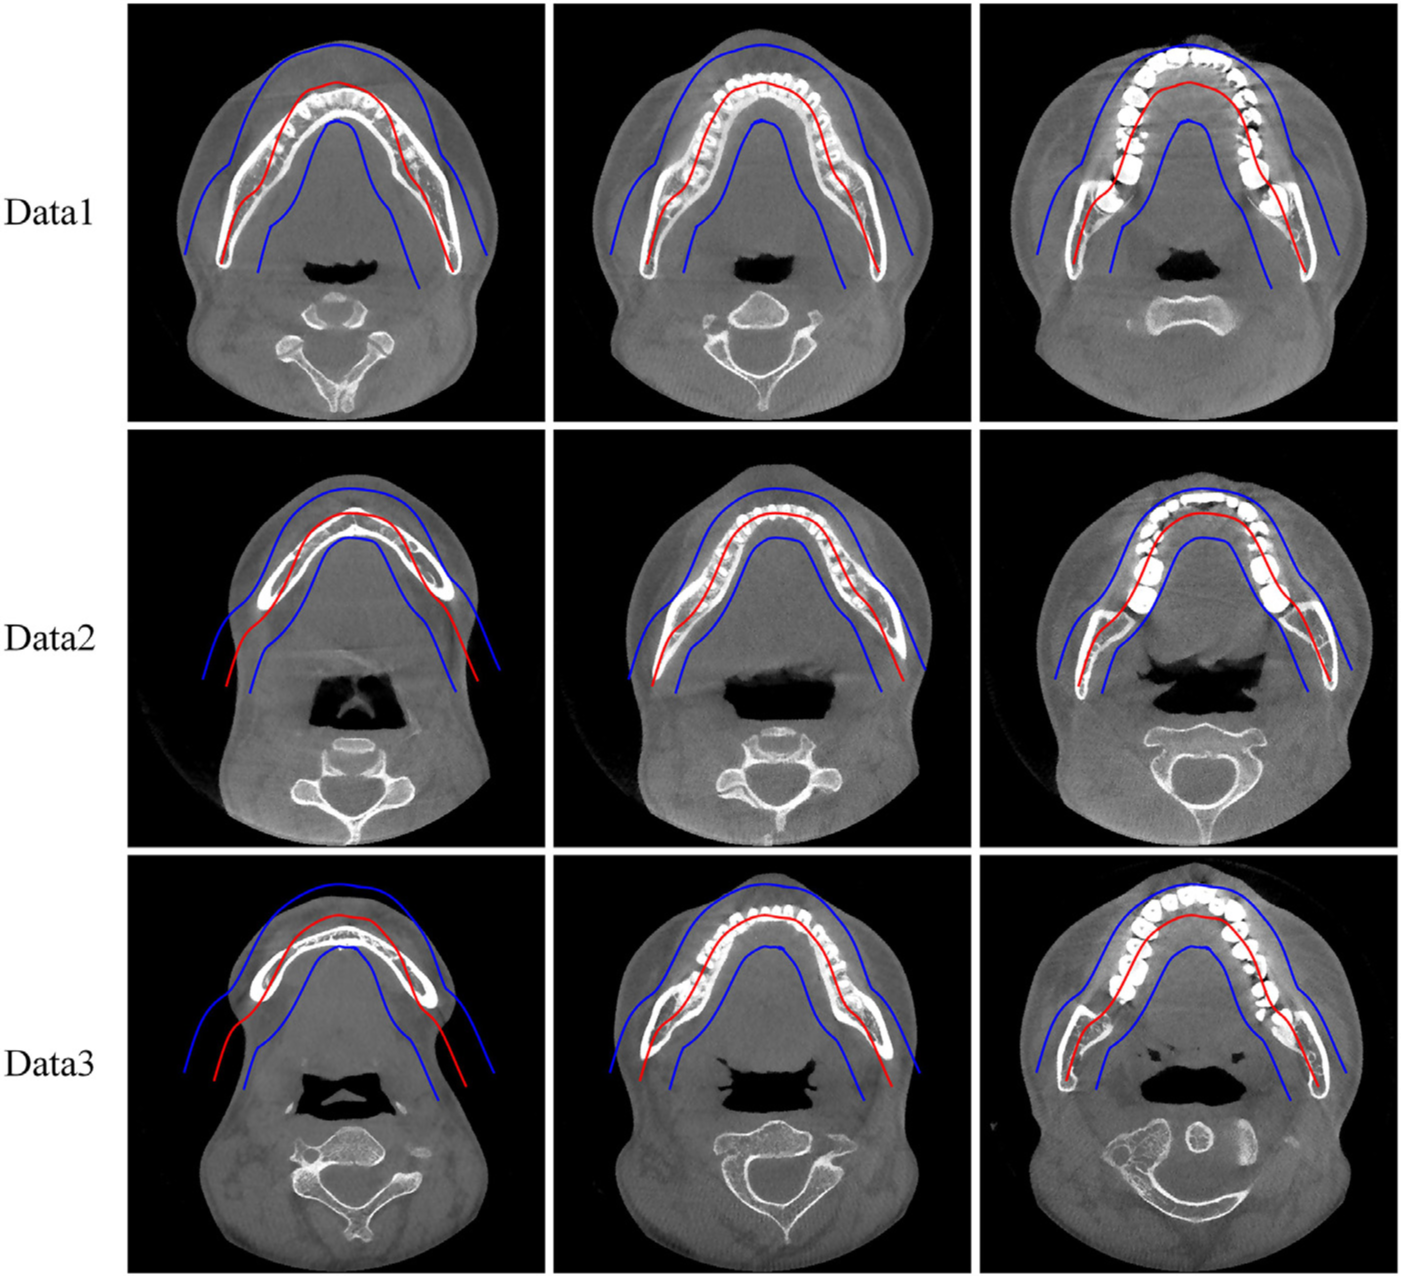
\includegraphics[width=0.7\textwidth]{img/dental_arch.png}
    \end{figure}
\end{frame}


\begin{frame}{\secname}{Panoramic images generation}
    Using homographies and the arch estimation in each tooth, they are able to reconstruct a panoramic image of the whole teething.
    \begin{figure}
        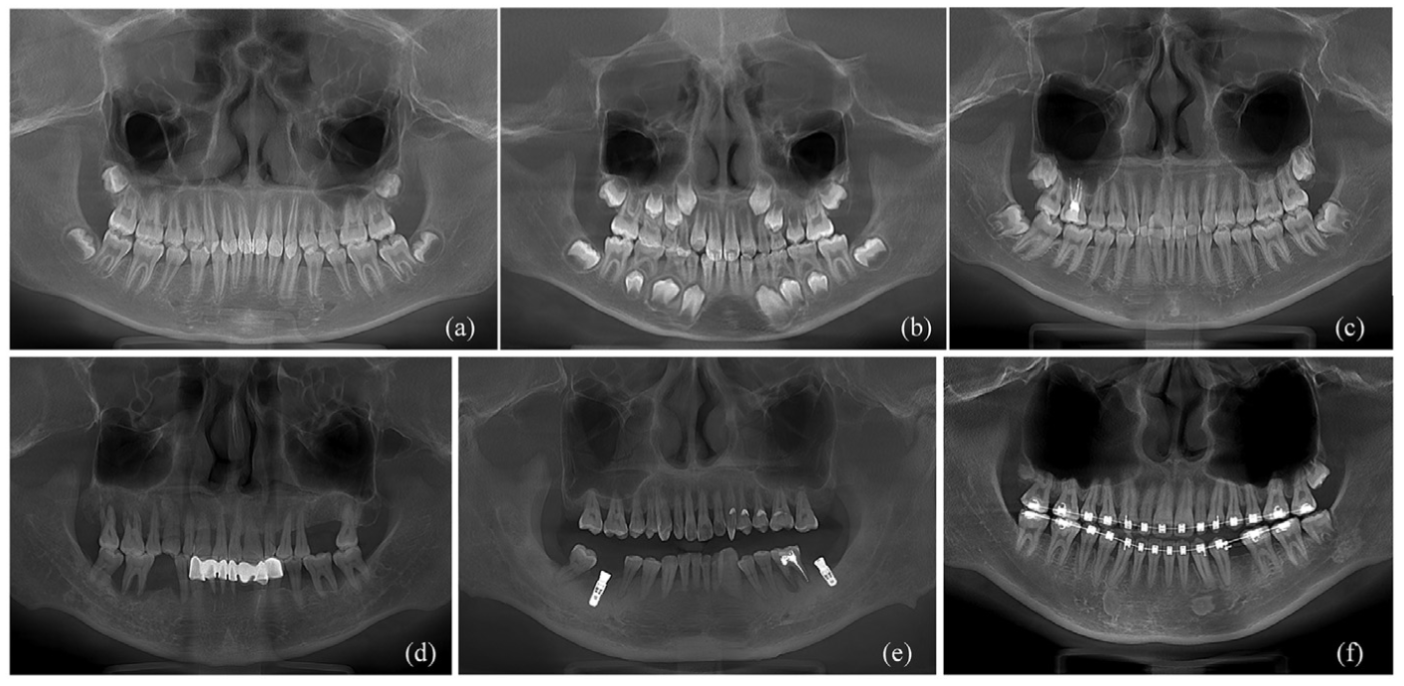
\includegraphics[width=\textwidth]{img/dental_pano}
    \end{figure}
\end{frame}

\begin{frame}{\secname}{Applications}
    Using techniques similar as the ones seen during the lessons, dentists can obtain automatic tooth identification.
    \begin{figure}
        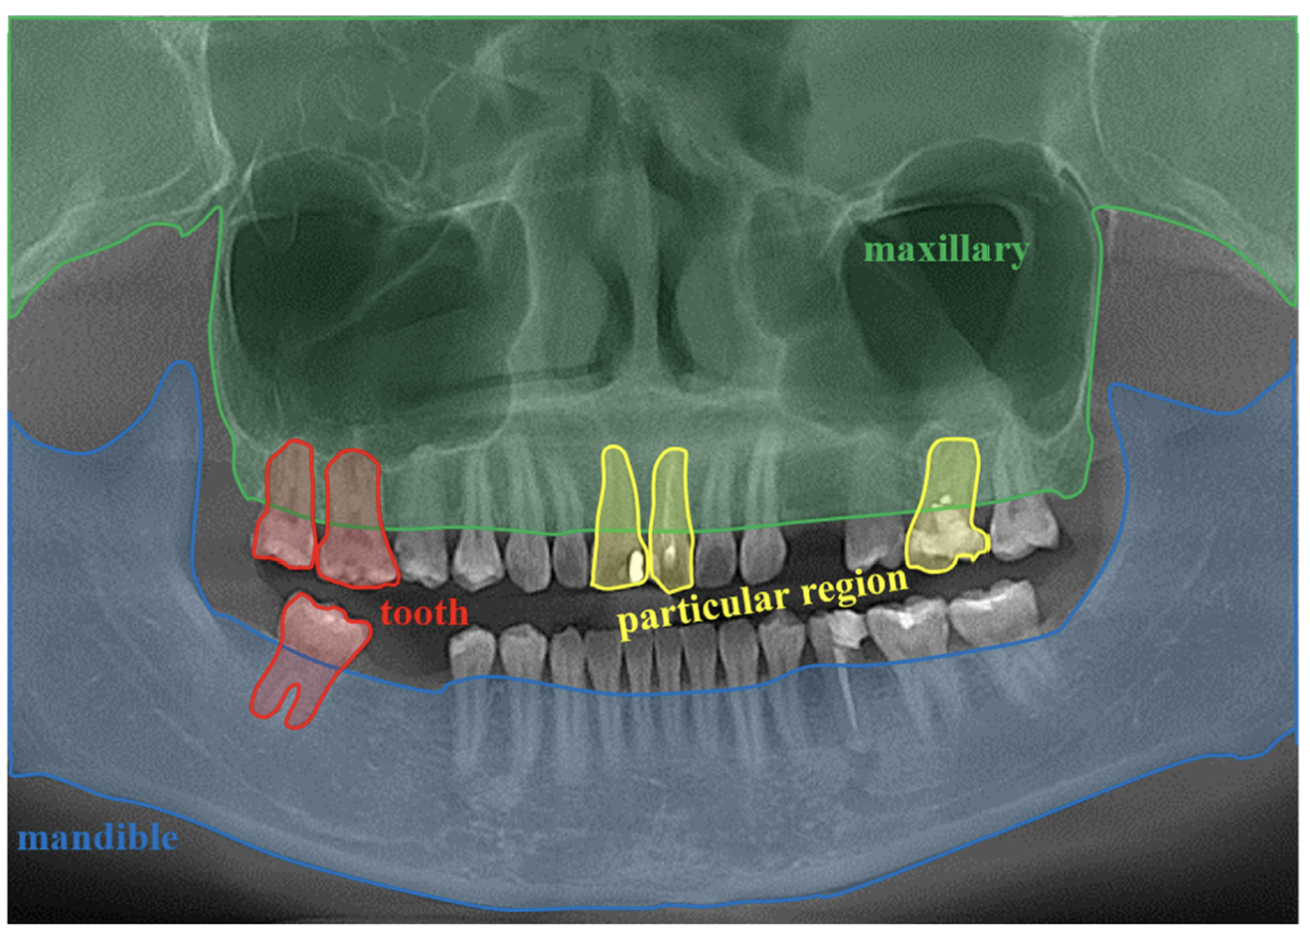
\includegraphics[width=0.5\textwidth]{img/dental_segmentation}
    \end{figure}
\end{frame}

\begin{frame}{\secname}{Known problems}
    One future path of this method is dealing with mental objects.
    \begin{figure}
        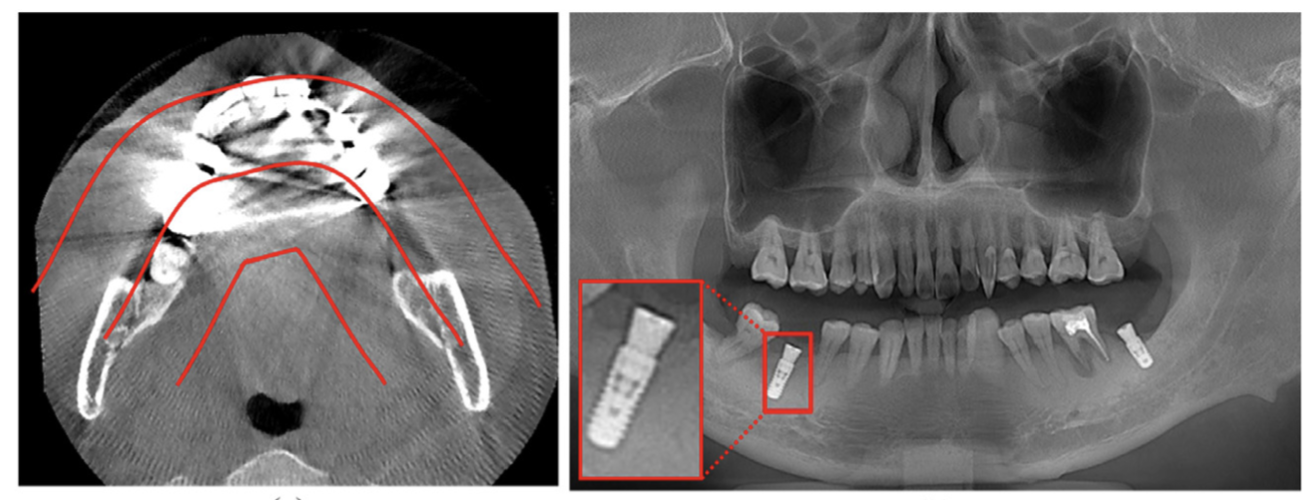
\includegraphics[width=0.7\textwidth]{img/dental_method_problems}
    \end{figure}
\end{frame}


\section{References}

\begin{frame}[allowframebreaks]{References}
    \nocite{*}
    \printbibliography
\end{frame}

\end{document}
